% A4 lap méret, 12 pontos betűméret
\documentclass[a4paper,12pt]{article}

% szükséges csomagok importálása
\usepackage[utf8]{inputenc}
\usepackage[T1]{fontenc}
\usepackage[magyar,english]{babel}
\usepackage{float}
\usepackage{lmodern}
\usepackage{graphicx}
\usepackage{pdfpages}
\usepackage{caption}
\usepackage[colorlinks=false, pdfborder={0 0 0}, linkcolor=black, unicode]{hyperref}
\usepackage{subcaption}
\usepackage{mathtools}
\usepackage{relsize}
\usepackage{amsmath}
\usepackage{amsfonts}
\usepackage{amssymb}
\usepackage{listings}
\usepackage{csquotes}
\usepackage{enumitem}
\usepackage{url}
\usepackage[nottoc,numbib]{tocbibind}
\usepackage{titlesec}
\usepackage{titletoc}
\usepackage{setspace}
\usepackage{fancyhdr}
\usepackage{setspace}
\usepackage{tocloft}
\usepackage[numbers]{natbib}
\usepackage{afterpage}
\usepackage{xcolor}
\usepackage{listings}

% Oldal margók beállítása
\usepackage[left=2.5cm, bottom=2.5cm, left=3cm, right=2cm]{geometry}

% Beállítások a hyperref csomaghoz
\hypersetup{
	colorlinks=true,
	linkcolor=blue,
	filecolor=magenta,      
	urlcolor=cyan,
}

% Címoldal beállítása
\title{\textbf{Szakdolgozat}}
\author{Mózer Viktor}
\date{Dátum}

% Oldalfejléc beállítása
\pagestyle{fancy}
\fancyhf{}
\fancyfoot[C]{\thepage}
%\renewcommand{\footrulewidth}{0pt}	%lábjegyzet vonal beállítás
\renewcommand{\headrulewidth}{0pt}	%fejléc vonal beállítás

% Szöveg beállítások
\setstretch{1.5}
\setlength{\parindent}{0pt}
\setlength{\parskip}{12pt}

% Rész-fejezet címsorok formátumának beállításas
%\setcounter{secnumdepth}{3}
\titleformat{\section}
	{\clearpage\normalfont\huge\bfseries}{\thesection.}{0.5em}{\huge}
	

%\titleformat*{\section}{{\clearpage\normalfont\huge\bfseries}{}{0em}{\huge}}

%{\típus  }{betűtípus\betűméret\vastag betűtípus}{margók}{bekezdés behúzása}\normalfont

% Dolgozat címe [Thesis title]
\def\thesisTitle{DIGITÁLIS HULLÁMFORMA GENERÁTOR MEGVALÓSÍTÁSA ÉS MÉRÉSE FPGA KÖRNYEZETBEN}

%Tartalomjegyzék formázása
\renewcommand{\contentsname}{\small Tartalomjegyzék}	%kisebb betűkS
\setlength{\cftbeforetoctitleskip}{0pt}					
\renewcommand{\cftdotsep}{0.5}			

%Irodalomjegyzék formázása
\bibliographystyle{plain} 

%Ábrák formázása
\counterwithin{figure}{section} % Ábrák számozása a szekció sorszáma szerint
\DeclareCaptionFormat{myformat}{\textbf{#1#2}#3\par}
\captionsetup[figure]{format=myformat}
%Ábák és képek a fig mappában
\graphicspath{{fig/}}
%----------------------------------------------------------------------
% Dokumentum kezdete
\begin{document}

	%\pagestyle{empty}	%fejléc levétele
	\selectlanguage{magyar}
	\pagenumbering{gobble} %nem számozott
	
	% Címoldal
	\begin{titlepage}
		\begin{center}
			\vspace{1em}
			\textbf{Budapesti Műszaki és Gazdaságtudományi Egyetem}\\
			Villamosmérnöki és Informatikai Kar\\
			Elektronikus Eszközök Tanszék
			
			\vspace*{3cm}
			
			\textbf{\huge Szakdolgozat}
			
			\vspace{1.5cm}
			
			\textbf{\large \thesisTitle}
			
			\vfill
			
			\vspace{0.8cm}
			
			%borítókép
\begin{figure}
	\centering
	
\includegraphics[width=0.7\linewidth]{bme_logo_kicsi}
	%\caption{}
	\label{fig:bmelogokicsi}
\end{figure}
		
			\vspace{3cm}
			
			%Konzulens, dátum, stb
			Készítette: Mózer Viktor (QUEQEO)\\	
			Konzulens: Dr.~Horváth Péter\\
			BUDAPEST, 2023
			
		\end{center}
	\end{titlepage}

	%Tartalomjegyzék, ábrajegyzék, táblajegyzék:
	\tableofcontents\vfill
	%\listoffigures
	%\listoftables
%----------------------------------------------------------------------
	\clearpage
	\phantomsection
	\addcontentsline{toc}{section}{Kivonat}
	\section*{Kivonat}
	Az elektronikában gyakran használnak perdiodikus jeleket különböző mérésekre, kommunikációra, jelfeldolgozásra stb. Ezeket a periodikus jeleket különféle analóg vagy digitális függvénygenerátorokkal állítják elő. Ebben a dolgozatban egy digitális elven működő hullámforma generátor tervezését és megvalósítását mutatom be FPGA (Field Programmable Gate Arrays) környezetben. Ezen eszköz segítségével lehetővé válik különböző típusú -és frekvenciájú jelek előállítása. A tervezett rendszer a Direct Digital Synthesizer (DDS) módszeren alapul, amelynek lényege, hogy egy numerikus vezérlő segítségével állíthatjuk elő a kívánt jeleket. A DDS módszerrel könnyen és rugalmasan generálhatók a különböző típusú jelek, például szinusz, négyszög vagy háromszög hullámformák, valamint azok frekvenciái is könnyen és gyorsan állíthatók. A tervezett rendszert számítógépen keresztül lehet vezérelni és beállítani a megjeleníteni kívánt hullámforma adatait. A dolgozatban bemutatom a tervezési folyamatot, a rendszer architektúráját, a hardver- és szoftver megvalósítását, valamint az eszközön elvégzett különböző mérések eredményeit, a rendszer teljesítményét. A tervezett digitális hullámforma generátor nagy pontossággal és stabilan képes generálni a különböző típusú és frekvenciájú jeleket, így széles körű alkalmazási lehetőséget kínál a digitális jelszintézis területén.

	\pagenumbering{roman}
	\selectlanguage{english}
	\clearpage
	\phantomsection
	\addcontentsline{toc}{section}{Abstract}
	\section*{Abstract} 
	Periodic signals are often used in electronics for various measurements, communications, signal processing, and so on. These periodic signals are generated using different analog or digital function generators. This paper presents the design and implementation of a digital waveform generator based on FPGA (Field Programmable Gate Arrays) technology. This device enables the production of various types and frequencies of signals. The designed system is based on the Direct Digital Synthesizer (DDS) method, which uses a numerical controller to generate the desired signals. The DDS method allows for easy and flexible generation of various types of signals, such as sine, square or triangular waveforms, and their frequencies can also be freely adjusted. The designed system can be controlled and adjusted via a computer to display the desired waveform data. This thesis presents the design process, system architecture, hardware, and software implementation, as well as the results of various measurements performed on the device and its performance. The designed digital waveform generator can generate various types and frequencies of signals with high accuracy and stability, thus offering a wide range of application possibilities in the field of digital signal synthesis.
	\selectlanguage{magyar}
	\newpage
	\pagenumbering{arabic}
	% Bevezetés
	\section{Bevezetés}
		A függvénygenerátorok olyan elektronikai eszközök, amelyek használhatók periodikus jelek, általában szinuszos hullámformák előállítására. Ezek az eszközök fontos szerepet játszanak a jelgenerálásban és a tesztelésben számos iparágban, beleértve az elektronikát, a kommunikációt, a hang- és videótechnikát, az optikát, az orvosi képalkotást, a tudományos kutatást és még sok más területet.
		Az elektronikában a függvénygenerátorokat általában a következőkben használják:
		\begin{itemize}
		\item Az oszcilloszkópok és spektrumanalizátorok kalibrálására és tesztelésére.
		\item A hang- és videótechnikában hullámformák és frekvenciák előállítására és tesztelésére.
		\item A kommunikációs rendszerekben digitális és analóg jelek előállítására és tesztelésére.
		\item Az orvosi képalkotásban a mágneses rezonancia (MRI) és az ultrahang vizsgálatokhoz használják a kívánt frekvenciák előállításához.
		\end{itemize}
	
		A függvénygenerátorokkal különböző hullámformákat és frekvenciákat lehet előállítani, amelyek lehetővé teszik a jellemzők és a teljesítmény tesztelését. Ezenkívül ezek az eszközök lehetővé teszik a jellemzők beállítását is, például a frekvencia, az amplitúdó és a fáziskésleltetés. Ez lehetővé teszi a felhasználók számára, hogy finomhangolják a jelet a kívánt specifikációkhoz és az adott alkalmazáshoz.
		
		A függvénygenerátorok általában két fő részből állnak: az oszcillátor áramkörből és az adó áramkörből. Az oszcillátor áramkör felelős a stabil és pontos alapjel előállításáért, míg az adó áramkör a szükséges jelalak előállítását végzi a kívánt frekvencia, amplitúdó és fázis beállítása mellett. 
		
		A jelgenerátorok megvalósíthatóak analóg -és digitális áramkörrel egyaránt. Előbbihez tartozik például a PLL, vagyis a fáziszárt hurok elvén működő generátor [1]. Utóbbiak közül egyik széles körben használt megoldás az úgynevezett Direct Digital Synthesis [2], röviden DDS elven működő generátor, melynek működése, tervezése és mérése jelen dolgozat témája is. A digitális hullámformák előállítása számos alkalmazási területen fontos szerepet játszik. Analóg szűrők és erősítők tesztelésekor szükséges számos fajta bemenő jelet előállítani, mint például szinusz, négyszög, háromszög hullámformákat. Emellett a digitális jelgenerátorok használhatók műsorszóráshoz, diagnosztikai alkalmazásokhoz, hangfrekvenciás vizsgálatokhoz és egyéb mérési feladatokhoz is.		
		
		A DDS generátor előállítására többféle megoldás létezik, például használhatunk integrált áramköröket (IC), mikrovezérlőket vagy programozható logikai áramköröket. Ezek közül az egyik legelterjedtebb típus az FPGA [3], mely digitális logikai áramkörök tervezésére és megvalósítására alkalmas. Az FPGA rugalmassága és nagy sebessége miatt a digitális jelgenerátorok tervezése és megvalósítása kiválóan megoldható vele.
		
		\subsection{Történelmi áttekintés, motivációk}
		Az 1960-as években megjelentek az első digitális hullámforma generátorok a műszeriparban, melyek azóta folyamatosan fejlődnek és bővülnek az alkalmazási területeik. Kezdetben az adatfeldolgozó iparban és a haderőnél használták őket, hogy teszteljék a digitális áramköröket és az elektronikai rendszereket. Az 1980-as évektől az iparban az analóg hullámformák digitális szintézisét alkalmazzák, amely lehetővé teszi a bonyolultabb hullámformák előállítását és programozását.
		A 90-es években a számítógépes technológia további fejlődése lehetővé tette a digitális hullámformák nagyobb pontosságú előállítását és a generátorok programozásának egyszerűsítését. Az elmúlt években a digitális hullámforma generátorok további fejlesztései lehetővé tették a nagyobb frekvencia-tartományok, a nagyobb pontosság és a nagyobb jelzaj arány elérését.
		A digitális hullámforma generátorok története folyamatosan bővül új fejlesztésekkel és technológiákkal. Az új technológiák előretörése és a fejlődő alkalmazások pedig újabb lehetőségeket nyújtanak a digitális hullámforma generátorok számára. Fontos megemlíteni, hogy ezek a generátorok jelentős szerepet játszanak a kutatásban, az oktatásban, az iparban és a mindennapi életünkben is. A további fejlesztések és kutatások pedig elősegíthetik az alkalmazási területek még szélesebb körű kiterjesztését.
			
		\subsection{A feladat célja}
		A feladatom célja egy DDS (Direct Digital Synthesis) elven működő digitális hullámformagenerátor tervezése volt, amelynek képessége kellő rugalmasságot biztosít a megfelelő jelek előállításához. Az eszköz az 20 Hz és 20 kHz közötti frekvenciatartományban képes megfelelő jel-zaj viszonyú, változtatható dinamikatartományú jelek előállítására, amelyek alkalmazási területek széles spektrumában használhatóak, mint például a hangfeldolgozás, akusztikai mérések vagy akár az orvosi diagnosztika. A tervezést FPGA technológiával valósítom meg.
		A DDS elvű jelgenerátor az egyik legelterjedtebb módszer a hullámformák digitális előállítására. Az elv alapja egy digitális szinusz hullámforma előállítása, melyet egy Digitális-Analóg konverterrel alakítunk át analóg jellé. A generálási folyamat során a frekvenciát és a fázist digitálisan állítjuk be, ami nagy pontosságot és stabilitást biztosít a generált jelben. Az előnyei közé tartozik az egyszerűsége, a nagy pontossága, a nagy dinamikatartománya és a rugalmassága. A DDS technológia számos alkalmazásban hasznos, különösen olyan területeken, ahol a frekvencia stabilizálása és a pontos hullámforma szükséges. A dolgozatomban ezt az elvet választottam, mivel célom volt egy olyan eszköz tervezése, amely magas frekvenciájú alkalmazásokban is használható, és amely nagy stabilitással és pontossággal generál jel-zaj viszonyban változtatható hullámformákat.
		A szakdolgozatom célja a tervezett digitális hullámformagenerátor megfelelő működésének biztosítása, amelyet előre meghatározott minőségbiztosítási feltételekkel ellenőrzök és mérésekkel igazolok. A minőségbiztosítási feltételeknek megfelelő működés biztosítása érdekében számos paramétert figyelembe veszek, mint például az amplitúdó pontossága, frekvencia stabilitása, jel-zaj aránya és a dinamikatartomány szélessége. Az elkészült eszköz teljesítményét alapos mérésekkel igazolom, amelyek magukba foglalják az amplitúdó és frekvencia stabilitás vizsgálatát, a dinamikatartomány mérését és a jel-zaj arány ellenőrzését.
		A dolgozat többi részében részletesen bemutatom a tervezett digitális hullámformagenerátor működését és felépítését, a tervezési folyamatot, az FPGA technológiát és az áramkörök tervezési lépéseit. Emellett részletesen bemutatom a mérések elvégzésének módszereit és a kapott eredményeket.
	
			
		\subsection{A dolgozat szerkezete}
		Bemutatom a generátor tervezési folyamatát, a szükséges hardveres eszközöket és az FPGA használatát. Emellett részletesen foglalkozom a tervezett hullámformák előállítását és azok mérését. A tervezett eszköz nagyfrekvenciás alkalmazásokban hasznos, például analóg szűrők és erősítők tesztelése során.
		A dolgozat első részében megvizsgáltam, hogy hogyan épül fel és mire használható egy DDS jelgenerátor. Továbbá megismerkedtem azzal az eszköztárral, amelyek segítségével garantálni tudom a megfelelő működést. 
		A következő fejezetben meghatároztam a rendszer működésének feltételeit és hogy a generált hullámforma milyen jellemzőkkel rendelkezzen, például jel-zaj viszony, dinamikatartomány stb.
		Ezután a rendszertervezés fázisa következett, ahol a mind a hardvert, mind a szoftvert megterveztem és megvalósítottam. A hardver- és szoftver különálló tesztelése után összakapcsoltam a két egységet és együtt teszteltem a rendszer megfelelő működését. 
		Végül mérésekkel igazoltam, hogy a generátor megfelel-e az előre meghatározott kritériumoknak. Az eredményeket lásd ~\apageref{sec:Összefoglaló}.~oldalon.

	\newpage
	%Fejezetek
%----------------------------------------------------------------------
	%\setcounter{section}{0}
	\section{Irodalomkutatás}
	
		\subsection{Közvetlen Digitális Szintézis elve}
		A Direct Digital Synthesis (röviden DDS), magyarul Közvetlen Digitális Szintézis egy módszer, mely analóg jelek előállítására szolgál digitális technológia segítségével. Általában szinusz hullámok előállítására használják, de előállítható vele akár négyszög- és háromszögjel is. Teszi mindezt úgy, hogy először egy időben változó digitális jelet állít elő, majd ezt egy digitál-analóg átalakítóval analóg jellé alakítja. Ezen technika ma már széles körben használt és a technológia fejlődésével alacsony fogyasztású, nagy megbízhatóságú és gyors működésű jelgenerátorokat képesek előállítani.
		\subsection{A DDS működése}
			Egy ilyen elven működő hullámforma generátor jellemzően három fő részből áll.
			Egy fázisakkumulátor vagy fázis-összeadó áramkörből, egy fázis-amplitúdókonverziós részből, mely jellemzően egy szinusz tábla vagyis egy memória, ami egy 1 periódusnyi szinusz hullám mintavételezett amplitúdóértékeivel van fetöltve. Ezeket együttesen nevezzük Numerically Controlled Oscillator-nak, rövid NCO-nak. Ez gyakorlatilag egy digitális periodikus jelet állít elő, innen tehát a neve. A rendszer továbbá áll egy digitál-analóg átalakítóból, ami az NCO által előállított digitális hullámformát alakítja át analóg jellé, ennek kimenetén sokszor egy aluláteresztő szűrő található, ami kiszűri a magas frekvenciájú felharmonikusokat, ezáltal javítva a jel minőségét.
			Továbbá az áramkör tartalmaz egy belső referencia órajelet is, mely azt adja meg, hogy milyen időközönként veszünk mintát a tárolt adatokból, ez általában a rendszer órajele.
			A fázisakkumulátor egy úgynevezett “adatszót” (tunning word) kap, mely megadja, hogy a fázisakkumulátor mekkora “lépésekkel” menjen végig a szinusz táblán. Gyakrolatilag ez határozza meg a kimeneti frekvenciát. Erről részletesen a következő alfejezetben írok. Az áramkör még tartalmazhat profil regisztereket, melyek előre beprogramozott regiszterek, ezekben be lehet állítani a frekvenciát, fázist, interpolációt és még sok más értéket.
			
			\begin{figure}[h!]   %[] a kép pozíciója, h! ahova írva van a kódban ott jelenjen meg
				\centering
				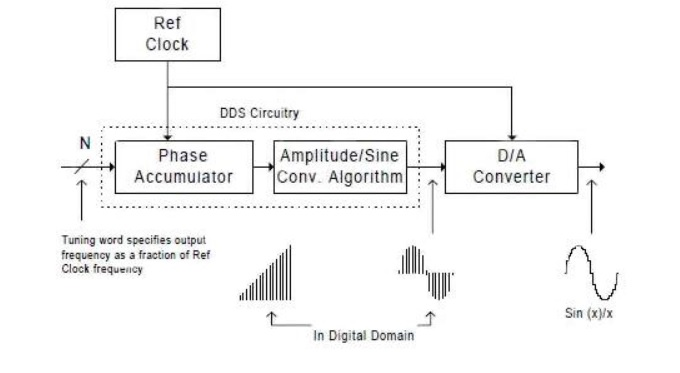
\includegraphics[width=10cm]{fig1.jpg}
				\caption{A DDS generátorműködését szemléltető ábra\cite{dds_principles_fig1}}
			\end{figure}
			\subsubsection{Fázisakkumulálás:}
			Adott egy folytonos idejű hullámforma, legyen ez most egy szinuszhullám. Ezt a következőképpen írjuk le:
			$u(t)=\sin(\theta)$
			Ennek fázisát ($\theta$) egy $0$-tól $2\pi$-ig terjedő szöggel lehet leírni. A digitális jelet szintén le lehet írni így viszont ilyenkor csak diszkrét értékeket vehetnek fel ezek a szögek. Ezt a következő digitális fáziskör ábrával tudjuk reprezentálni.
		
			\begin{figure}[h!]   %[] a kép pozíciója, h! ahova írva van a kódban ott jelenjen meg
				\centering
				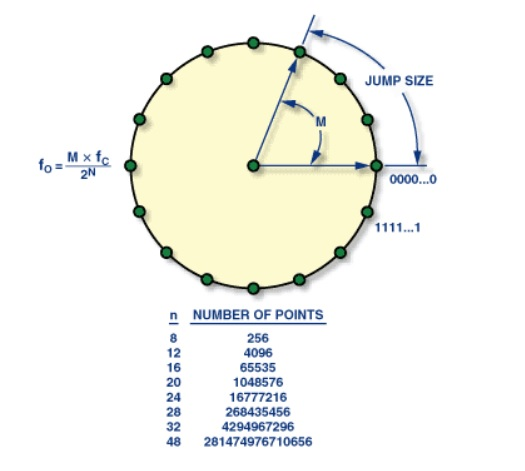
\includegraphics[width=10cm]{fig2.jpg}
				\caption{Fázis vektor diagram\cite{phase_wheel_fig2}}
			\end{figure}
		
			Adott egy vektor melynek kezdőpontja a kör középpontjától és végig a kör mentén mozog adott sebességgel, amint véget ért egy kör, vagyis $0$-tól $2\pi$ -ig, akkor indul előről. Ez tehát egy folyamatosan futó szinuszhullámot jelent. Ezen digitális szinusz adatait egy memóriába tároljuk el és ezen a memórián egy számlálóval tudunk végigmenni, mely ha túlcsordul újrakezdődik a számlálás. 
			Ez a számláló a bemenetére kap egy már az előbbiekben említett adatszót (tunning word), ezt legtöbbször M betűvel jelöljük, ez a szó egy bináris számnak felel meg. Ezzel állítjuk a frekvenciát mégpedig úgy, hogy a számlálóhoz mindig ezt a számot adjuk hozzá, ez azt eredményezi, hogy minden egyes belső órajelre ennyit lépünk a szinusz táblában. Így hamarabb végig érünk az adatokon, vagyis a frekvenciánk nagyobb lesz. Azonban mivel kevesebb adatból veszünk mintát a felbontásunk is kisebb lesz. 
			Ezt a következő ábra szemlélteti, amin látszik ez a szó (M) és maga a számláló, amit itt “phase register” névvel jelöltek. Ez folyamatosan címzi a szinusz táblát, itt “Phase-to-Amplitude Converter”.
			\begin{figure}[h!]   %[] a kép pozíciója, h! ahova írva van a kódban ott jelenjen meg
				\centering
				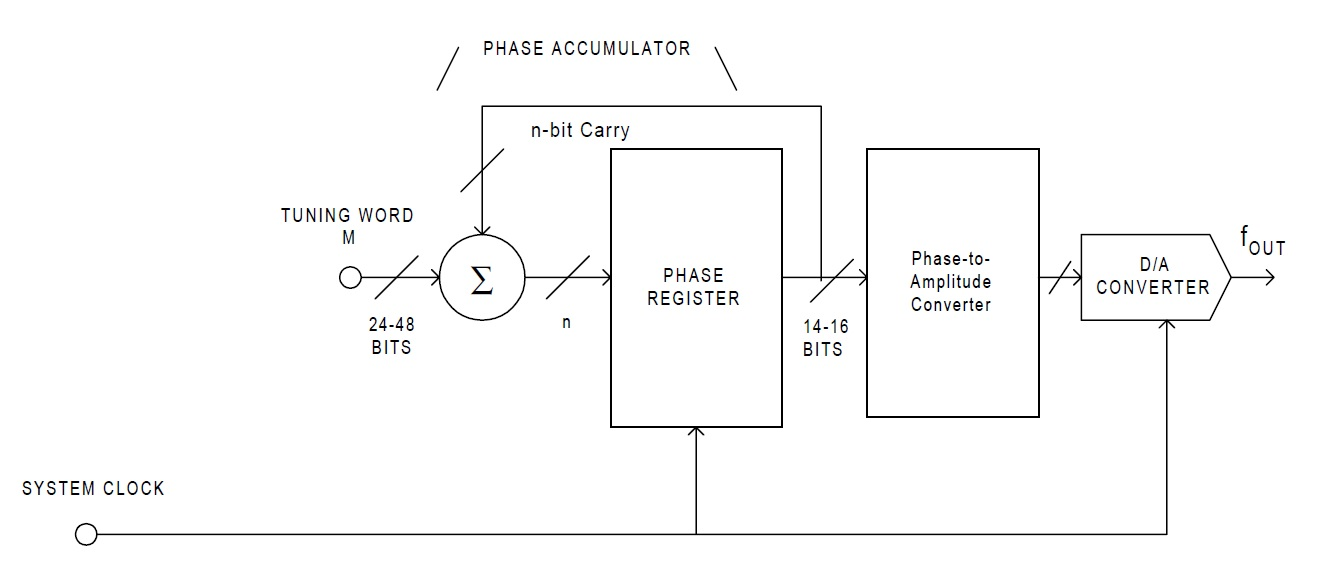
\includegraphics[width=10cm]{fig3.jpg}
				\caption{Fázisakkumulátor\cite{dds_phase_accu_fig3}}
			\end{figure}
			
			A kimeneti frekvencia a következő összefüggés segítségével számítható:
			\begin{center}
			$ f_{out} = \frac{M \times f_{C}}{2^n}$
			\end{center}
			Ahol:
			\begin{itemize}
				\item $f_{out}$ a kimeneti frekvencia
				\item $M$ a bináris frekvencialépés
				\item $f_{C}$ beslő órajel
				\item $n$ a fázisakkumulátor bitjeinek száma
			\end{itemize}
			Tegyük fel, hogy adott egy $n=16$ bites fázisakkumulátorunk, vagyis $2^n=2^{16}=65\ 535$ értéket tárolunk az akkumulátorban.
			A minimális lépésköz (M) ‘1’ értéket vehet fel, ezáltal végigmegyünk minden egyes adaton. Ez a minimális frekvenciát és a maximális felbontást eredményezi.
			Ha M ’32768’ értéket veheti fel, akkor két órajel ciklus után túl is csordul a számlálónk. Azonban a mintavételi törvény kimondja, hogy egy mintavett jel akkor és csak akkor 
			rekonstruálható a mintáiból, ha a jel frekvenciatartománya (maximális frekvencia) nem nagyobb a mintavételezési frekvencia felénél. Képlettel felírva ez annyit tesz, hogy:
			\begin{center}
			$f\leq\frac{f_{s}}{2}$ 
			\end{center}
			Jelen példánkra kiszámítható, hogy a maximálisan megengedhető lépésköz:
			\begin{center}
			$\frac{f_{s}}{2}=\frac{M\ast f_{s}}{2^{16}}\Rightarrow M=32\ 768$
			\end{center}
			A következő ábrán jól szemléltethető a frekvencia változtatása. Analóg jelnél ezt úgy tesszük, hogy a szinusz függvény szögét minél nagyobbra választjuk.
			\begin{figure}[h!]   %[] a kép pozíciója, h! ahova írva van a kódban ott jelenjen meg
				\centering
				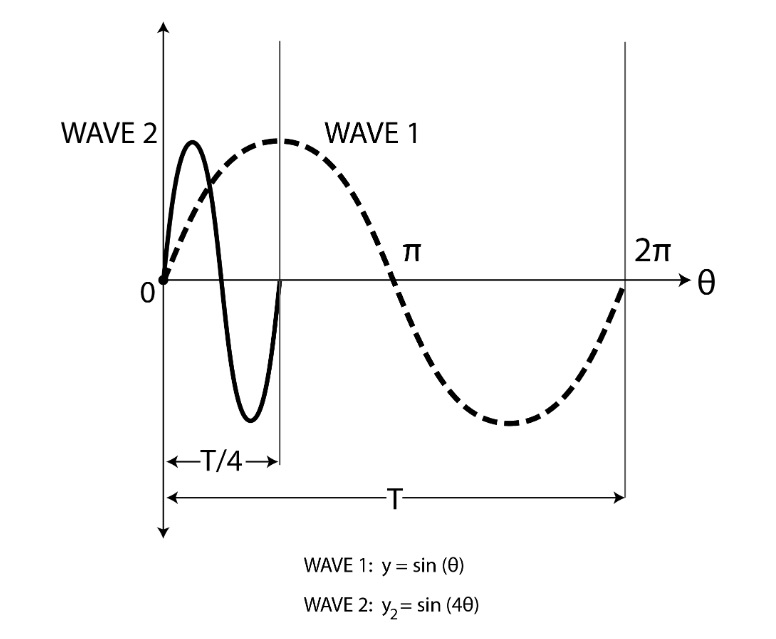
\includegraphics[width=10cm]{fig4.jpg}
				\caption{Frekvencia változtatása\cite{frequency_change_fig4}}
			\end{figure}
			Az ábrán látható, hogy ha 4-szer akkora a szög, akkor a periódus idő is negyede lesz az eredeti periódusidőnek. Digitális jelnél ugyanez a jelenség figyelhető meg, négyszer gyorsabban végig tud lépkedni a fázisakkumulátor az adatokon, mivel a lépésköz a négyszerese az eredetinek, ezért minden negyedik adaton megy csak végig. E szintén azt eredményezi, hogy T idő alatt kiadódik négy egész periódus szinuszjel.
			\newpage

			\subsection{DDS generátorok főbb tulajdonságai, mérésének elvei, jelfeldolgozás}
			Az egyik ilyen fontos tulajdonság a frekvenciahangoló szó vagy más néven tunning word. Erről az előző fejezetben szó volt, ennek segítségével beállíthatjuk a kimeneti frekvenciát. 
			Fontos tulajdonság továbbá a felbontás, amely a generált szinusz hullámforma frekvenciájának finomságát jelenti, vagyis a minimális frekvencia lépésközt. A felbontás meghatározza, hogy milyen pontosan állítható be a generált hullámforma frekvenciája. A felbontást általában a fázisakkumulátor bithossza határozza meg, ami a digitális jelfeldolgozás során használt legkisebb egységeket jelenti. Például legyen 14 bites ez a szó, tehát n=14, ekkor a kövekezőképpen tudunk számolni:
			\begin{center}
				$\Delta\theta = \frac{360^\circ \cdot 2}{2^n} =  \frac{360^\circ \cdot 2}{2^{14}} \approx 0.0439^\circ$
			\end{center}
			Tehát 0.0439 fokos fáziskésleltetési vezérlési felbontást biztosít nekünk ez a bitmélység.
			Abban az esetben, ha a rendszer órajele (SCLK) 50MHz és ebből szeretnék előállítani 96kHz mintavételi frekvenciájú (REFCLK) jelet, így a következő összefüggéssel lehet kiszámítani, hogy milyen szorzószámmal lehet létrehozni ezt a frekvenciát egy úgynevezett “strobe” áramkörrel:
			\begin{center}
				Szorzó = $\frac{SCLK}{REFCLK} = \frac{50MHz}{96kHZ} = 520$
			\end{center}
			Ilyenkor a kimeneti frekvencia sávszélessége (feltételezve a REFCLK ráta egyharmadát) 32kHz.
			
			\textbf{A Dinamikatartomány:} Az ideális DDS kimenetének lehetővé kell tennie a dinamikus tartományon belüli finomhangolást, illetve a kimeneti jel amplitúdójának változtatását. A dinamikai tartomány (angolul dynamic range) a minimális és maximális kimeneti amplitúdó értékek közötti különbséget jelenti. Tehát a dinamikai tartományt a két mért érték közötti különbséggel tudjuk meghatározni. Az analóg jelek dinamikatartományát az áramkörök, műszerek vagy érzékelők határozzák meg. Az adott rendszer dinamikatartománya lehetővé teszi az adott jelminőség hatékony érzékelését és feldolgozását. A digitális jelkezelésben a dinamikatartomány a digitális jelek bináris értékeinek legkisebb és legnagyobb értéke közötti különbséget jelöli.
			A DDS esetében a dinamikatartomány azt jelenti, hogy az általánosan használt referenciaóra (pl. kristályoszcillátor) hibái és a digitális jelek szintézisének zajai miatt mekkora különbséggel lehet generálni a kimeneti jelet a maximális és a minimális amplitúdó értékek között.
			A dinamikatartomány erősen függ az adott áramkör tervezésétől és a referenciaóra stabilitásától, valamint a digitális jelek szintézisének zajától és torzításától. A DDS esetében a magas dinamikatartomány nagyobb szabadságot ad a kimeneti jel generálásához, például nagyobb frekvenciatartomány lefedéséhez és jobb fázisstabilitáshoz vezet. 
			Azonban ha van jelen zaj, márpedig az esetek döntő többségében kell számolnunk némi zajjal, akkor az úgynevezett SFDR mérőszámot használjuk a dinamikatartomány megadására. A digitális jelgenerátorok dinamikatartományát általában ezzel az értékkel jellemzik.  
			Az SFDR rövidítés a "Spurious-Free Dynamic Range" kifejezésre utal, amely a jel/torzítás viszonyítási értékét jellemzi egy adott rendszerben. Az SFDR azt az értéket méri, hogy milyen nagy amplitúdójú lehet a legnagyobb hasznos jel, amelyet az adott rendszer tud előállítani, anélkül hogy a torzítások (vagyis a nemkívánatos mellékjelzések) elérnék a hasznos jel amplitúdóját. Ez megadja, hogy mekkora a legnagyobb (maximális szintű) jel és a legnagyobb zajszint közötti különbség. Az SFDR mértékegysége decibel (dB) és általában nagyobb értéke jelent jobb minőséget.
			A Spurious-Free Dynamic Range (SFDR) képlete a következő:
			\begin{center}
				$SFDR^{\mathrm{db}} = 20 \log_{10} \left( \frac{A}{B} \right)$\\
				$SFDR^{\mathrm{db}} = A^{\mathrm{dB}} - B^{\mathrm{dB}}$
			\end{center}
			, ahol A a jel maximális amplitúdója, és B a legmagasabb szintű “spur” vagyis a szennyező jel amplitúdója. Mindkét értéket ugyanabban az egységben kell kifejezni, például dBFS vagy dBmV. A spur az a jel, amely az általunk kívánt frekvencia többszörösén generálódik az ideális tiszta sinuszos jel helyett.
			Ezt a következő ábrán láthatjuk:
			\begin{figure}[h!]   %[] a kép pozíciója, h! ahova írva van a kódban ott jelenjen meg
				\centering
				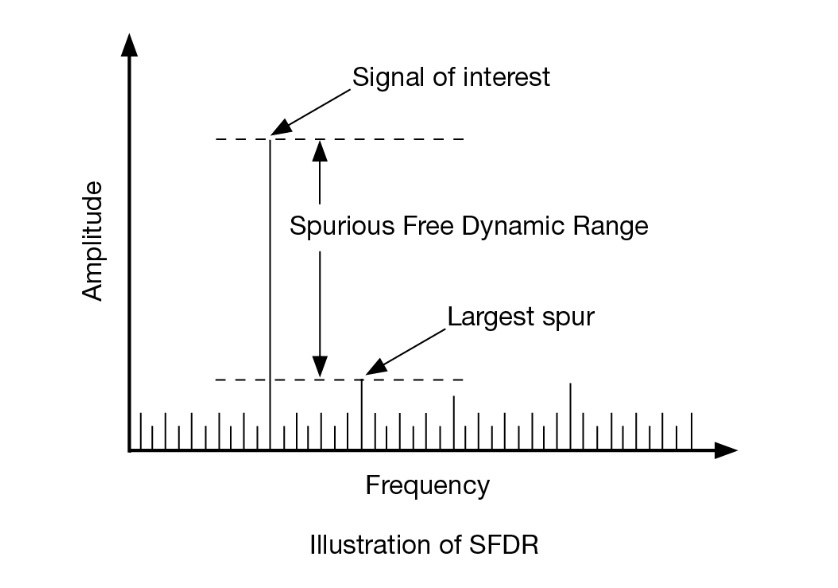
\includegraphics[width=10cm]{fig5.jpg}
				\caption{Spurious Free Dynamic Range\cite{sfdr_principle_fig5}}
			\end{figure}
			Az SFDR értéke fontos paraméter a DDS generátorok esetében, mivel ez határozza meg a generált jel minőségét, és a torzítások milyen mértékben szennyezik a hasznos jel spektrumát. Jellemző értéke 80dB. Egy jó SFDR-tel rendelkező DDS képes lesz arra, hogy előállítson egy nagyon tiszta spektrumot, amely szükséges például a digitális kommunikációs alkalmazásokban. 
			Egy DDS generátor esetén ki tudjuk számítani az NCO és a DAC SFDR érétkét is, és ezeket megfelelően összegezve megkapjuk a kimeneti jel SFDR tartományát.
			NCO dinamikatartomány:
			$Jel-zaj viszony^{\mathrm{dB}} = 6,02 dB * m + 1,76 dB$ 
			Itt m azt jelenti, hogy hány bites adatomvan.
			Az SFDR értéke a DAC zajszintjétől és az NCO dinamikatartományától függ. Ha a DAC zajszintje elhanyagolható, akkor az SFDR értékét az NCO dinamikatartományához hasonlóan számíthatjuk:
			$SFDR^{\mathrm{dBc}} = 20 * log (N) + SNR^{\mathrm{dBFS}} - 1,76 dB$
			Ahol N a nem kívánt spektrumkomponensek száma, SNR pedig a DAC-jel zajállósága.
			Azonban, ha a DAC zajszintje nem elhanyagolható, akkor figyelembe kell venni a DAC jel-zaj arányát is. Ha a DAC zajszintje $SNR_dBFS$ értékű, akkor az SFDR értéke az alábbi módon számolható:
			$SFDR^{\mathrm{dBc}}= 20 x log (N) + (SNR_dBFS - (6,02 x m + 1,76))  - 1,76 dB$
			Ahol N a nem kívánt spektrumkomponensek száma, $SNR_dBFS$ a DAC jel-zaj aránya (dBFS-ben), a bitmélység pedig a DAC és az NCO biteinek száma. A $min(0, SNR_dBFS - (6,02 * bitmélység + 1,76))$ a különbséget jelenti az NCO dinamikatartománya és a DAC jel-zaj aránya között, amely meghatározza az SFDR értékének korlátját.
			Az SFDR képletében az SNR értéke dBFS-ben van kifejezve, ami azt jelenti, hogy a jel-zaj arányt a teljes skálán lévő maximális értékhez, vagyis a teljes skála csúcsértékéhez viszonyítjuk. Ennek megfelelően az $SNR_dBFS$ értékét a következő képlettel lehet kiszámítani:
			$SNR_dBFS = 20 x log (A_jel / A_csúcs)$
			ahol $A_csúcs$ a DAC teljes skálán lévő csúcsértéke.
			Fontos megjegyezni, hogy az SFDR érték számítása és értéke nagyban függ az alkalmazott analóg és digitális áramkörök minőségétől, valamint a jel-zaj aránytól. Ezért az elméleti számítások és a gyakorlati eredmények között eltérés lehet.
			
			\textbf{A digitális jelgenerátorok fontos jellemzője még a jitter.} A digitális jel jellegzetes tulajdonsága, hogy a jelsorozat időzítése bizonytalan, a jelsorozat állapotváltásai a névleges időponthoz képest eltérnek. Ez a tulajdonság - amennyiben az eltérések rövid időtartamúak - a jitter (remegés, dzsitter), mely nem más mint egy nemkívánatos fázismoduláció. Amennyiben az eltérések lassan változnak akkor a jelenség neve wander (vándorlás). 
			\begin{figure}[h!]   %[] a kép pozíciója, h! ahova írva van a kódban ott jelenjen meg
				\centering
				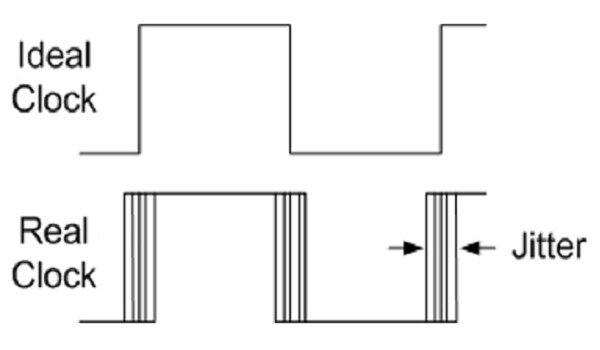
\includegraphics[width=10cm]{fig6.jpg}
				\caption{Jitter\cite{jitter_fig6}}
			\end{figure}
			A jittert általában szűrőkkel és időzítő áramkörökkel szűrik ki. A szűrőkkel a kimeneti jelet simábbá lehet tenni, míg az időzítő áramkörökkel biztosítani lehet a pontos időzítést. A pontos időzítés érdekében a DDS áramkörök gyakran tartalmaznak fáziszabályzókat és PLL (Phase Locked Loop) [] áramköröket is. Ha nem sikerül mérni a jittert, akkor a jel minőségének romlása lehet az eredménye, mivel a jitter hatással lehet a jel stabilitására és a zajszintre. Ha a rendelkezésre álló specifikációk nem elegendőek a jitter értékének meghatározásához, akkor a rendszer működése során mérési eredmények alapján kell meghatározni a jittert, és ennek figyelembevételével optimalizálni a rendszert. A jittert időben mért fázis-szórás segítségével lehet mérni, mely a következőképpen működik.
			A DDS jelgenerátor kimeneti jelének jitter-ét a periódusjitterrel (PJ) vagy a ciklusjitterrel (CJ) mérhetjük meg. A PJ az egyes periódusok közötti időeltéréseket méri, míg a CJ az egyes impulzusok közötti időeltéréseket méri.
			A jitter méréséhez szükségünk van egy precíz időmérő eszközre, mint például egy oscilloszkóp vagy időzítőmérő. A mérés során a DDS kimeneti jelének jelalakját és frekvenciáját hasonlítjuk össze az időzítőmérő jeleivel.
			A jitter mértéke általában ps (pikoszekundum) vagy fs (femtoszekundum) nagyságrendben adódik meg. A jitter mérésének pontosabb eredménye érdekében érdemes több mérési ciklust is végrehajtani és az eredményeket átlagolni.
		
			\textbf{Spektrum tisztasága:} A generátor spektrumának tisztasága jellemzően a generált jelekben jelenlévő nem kívánt spektrális komponensek (pl. harmonikusok, intermodulációs torzítás) szintjét jelenti.
			A spektrum tisztasága befolyásolhatja a generált jel minőségét, és fontos szerepet játszik az alkalmazásokban. Az intermodulációs torzítás (IMD) például akkor fordul elő, amikor két vagy több frekvenciát generálunk, amelyek nem egymás többszörösei. Az IMD torzítás csökkentése fontos, ha a generált jelet nagy dinamikatartományban vagy széles frekvenciaspektrumban használjuk.
			A spektrum tisztaságának meghatározása és javítása érdekében az alábbi lépéseket lehet tenni:
			\begin{itemize}
				\item{1} Az analóg kimenet szűrése:\\
				Az analóg szűrők használata csökkentheti a nem kívánt spektrális komponensek szintjét. Az analóg szűrők eltávolítják a nem kívánt komponenseket az analóg kimeneti jelből, és javítják a spektrum tisztaságát.
				\item{2} A generált frekvenciák helyes kiválasztása:\\
				A generált frekvenciák helyes kiválasztása fontos a spektrum tisztaságának javítása érdekében. Az IMD torzítás minimalizálása érdekében a generált frekvenciákat úgy kell kiválasztani, hogy azok egymás többszörösei legyenek.
				\item{3} Az NCO és DAC torzításának minimalizálása:\\
				Az NCO (Numerically Controlled Oscillator) és a DAC (Digital-to-Analog Converter) által okozott torzítások is hatással lehetnek a spektrum tisztaságára. A pontosabb NCO és DAC tervezése és alkalmazása javíthatja a spektrum tisztaságát.
			\end{itemize}
			A spektrum tisztaságának meghatározására használható mértékek közül a leggyakrabban használt a THD (Total Harmonic Distortion) és a SFDR (Spurious-Free Dynamic Range). A THD a generált jelben található összes harmonikus torzítás összegét jelenti, míg az SFDR az adott frekvencia spektrum legnagyobb jel-szintjének és a legnagyobb nem kívánt spektrális komponens szintjének a viszonya. A spektrum tisztaságának javítása érdekében ezeket a mértékeket minimalizálni kell. Én a dolgozatomban utóbbival (SFDR) foglalkozom.
			
			\textbf{Frekvencia stabilitás:} Az ideális DDS kimeneti jel frekvenciája stabil és pontosnak kell lennie. A frekvencia stabilitása és pontossága az időben mért frekvenciamérésekkel, illetve a frekvencia szabályozásával ellenőrizhető. 
			A frekvencia stabilitását a frekvencia drift és a fáziszaj paraméterrel szokták meghatározni.
			A frekvencia drift az időbeli frekvencia változás mértéke. Ez az érték általában pár ppm (parts per million) vagy pár száz ppm.
			A phase noise az időzítési jitter okozta frekvenciaspektrum zaj. Ez a jellemző határozza meg, hogy milyen mértékben jelennek meg a spektrumban az alapfrekvencia körüli zajkomponensek. A phase noise-t dBc/Hz-ben szokták megadni, ami azt jelenti, hogy az adott frekvencián belüli egy adott sávszélességre jutó teljesítmény az alapfrekvencia teljesítményének dB-ben kifejezett értékeivel van arányban.
					
			\subsection{D/A átalakító}		
			A digitális-analóg átalakító a bemeneti digitális adatoknak megfelelő analóg kimeneti jelet állítja elő. A kimeneti jel lehet feszültség vagy áram, de legtöbbször az áramkimenetű átalakítók jelét is feszültséggé alakítjuk. Az átalakításhoz szükség van egy fizikai referencia jelre, amely a digitális bemenetnek megfelelően átskálázva eredményez egy analóg kimeneti jelet. Ez általában egy referenciafeszültség, mely meghatározza a DA átalakító maximális és minimális kimeneti amplitúdóját. Minél stabilabb a referenciafeszültség, annál nagyobb a dinamikatartomány. A DA átalakítók még egy fontos jellemzője a bitmélység, ez azt jelenti, hogy a kimeneti amplitúdó nulla kimenettől a teljes skáláig hány lépésben érhető el. Például ha van egy 10 bites átalakítónk, akkor 1024 lépésben tehetjük ezt meg, vagyis 1024 feszültségszintet tudunk beállítani a referenciajel segítségével. Az átalakítókhoz szükséges még egy mintavételi frekvencia, mely a bemeneti jelből adott időközönként vesz mintát.
			A Digitális-analóg átalakítóknak sajnos zajuk is van, mely szintén szerepet játszik a dinamikatartomány méretében. A zaj csökkentése érdekében gyakran használnak szűrőket és egyéb zajcsökkentő módszereket. 
			Az átalakító adott időközönként mintát vesz a digitális adatokból és ezeket skálázza a megfelelő frekvenciaértékre. A mintavett adatokat megtartja a következő mintavételi iidőpontig (audió adatoknál ez jellemzően 44 és 96kHz). Ez látható az alábbi ábrán is. A két mintavételi pont között tartott adatot a különböző interpolációs technikával megvalósított kimeneti szűrők kisimítják. Így előáll egy analóg jel. 
			\begin{figure}[h!]   %[] a kép pozíciója, h! ahova írva van a kódban ott jelenjen meg
				\centering
				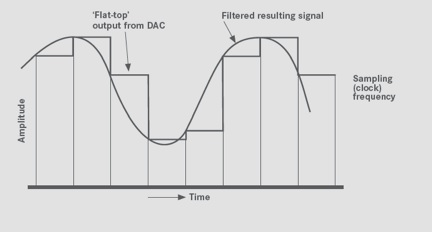
\includegraphics[width=10cm]{fig7.jpg}
				\caption{Spurious Free Dynamic Range\cite{dac_fig7}}
			\end{figure}

			A D/A átalakító tartalmaz: 
			\begin{itemize}
				\item \textbf{analóg kimenetet} (feszültség vagy áram), 
				\item \textbf{analóg referencia bemenetet} (ami lehet fizikailag külső, vagy már az IC-re integrált), amellyel a kimeneti jelet skálázza, 
				\item \textbf{digitális adatbemenet}, ahol az átalakítandó digitális kód megadható.
			\end{itemize}

			
	
			\subsection{FPGA-ra tervezés}
			A digitális rendszer tervezésének különböző elvonatkoztatási szintjeit az alábbi Gajski-Kuhn Y-diagram szemlélteti:
			\begin{figure}[h!]   %[] a kép pozíciója, h! ahova írva van a kódban ott jelenjen meg
				\centering
				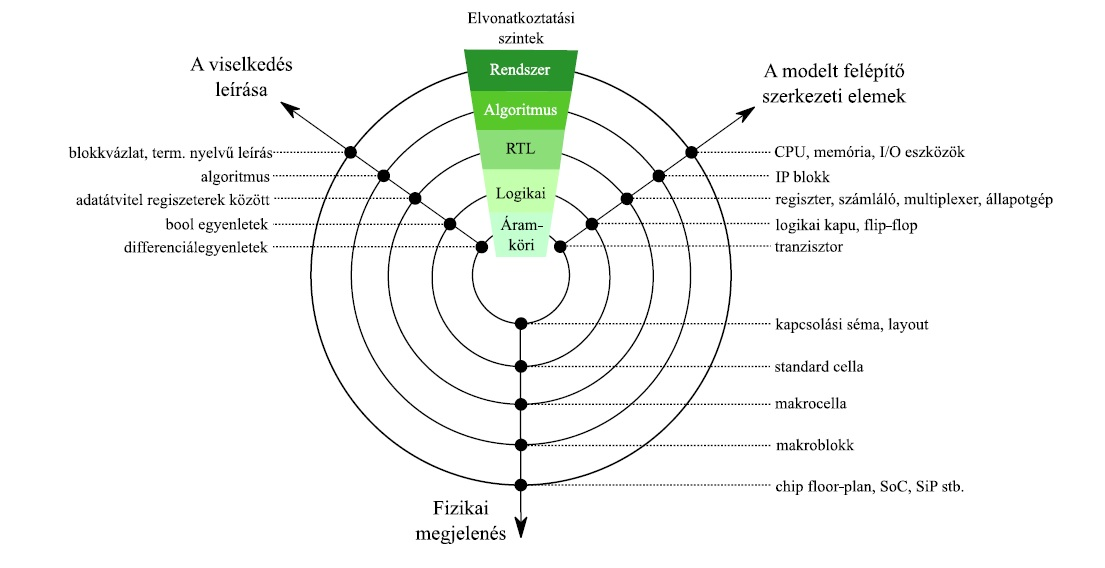
\includegraphics[width=10cm]{fig8.jpg}
				\caption{Gajski-Kuhn Y-diagram. A kép forrása \cite{gajski_fig8}}
			\end{figure}
		
			Először meg kell határoznunk a specifikáció alapján a rendszer interfészeit, működési tulajdonságait, stb. Itt megfigyelhető, hogy először a működési modellt állítjuk elő (algoritmus szint), jelen esetben generálunk egy megfelelő hullámformát. Ezután az RTL (Regsiter Transfer Level) tervezése következik, melyben megtervezésre kerül az RTL modell egyes almoduljainak működése és interfészei. Majd ezeket a modulokat integráljuk egy top level modulba, melyben az almodulok az interfészeiken keresztül kommunikálnak egymással. A helyes működést ellenőrizni is kell, ezt az úgynevezett verifikációval tesszük meg. Különböző verifikációs formákból, eljárásokból válogathatunk attól függően, hogy milyen alkalmazásról van szó, vagy milyen mélységben kell tesztelni az adott rendszert.  
			
			V\textbf{Verifikáció lépései:}Először a teszt környezetet építjük fel, amely tartalmazza az általunk tervezett rendszer modulját, melyet DUT-nak (Design Under Test) nevezünk. 
			Ezután tesztelési esteket és eljárásokat készítünk, amelyek előállítják a bemeneti adatokat, amelyeket a DUT-nak adunk át, ezek ellenőrzik a kimenetet, hogy megfelel-e a specifikációnak. Végül a teszt indításával és az eredmények ellenőrzésével zárjuk a folyamatot.
			
			Ezután következik az RTL szintézise, melyben a szintézis szoftver kialakítja az áramkör fizikai reprezentációját, melynek segítségével az FPGA-t konfigurálhatjuk fel. Itt figyelni kell arra, hogy a működés eltérhet a verifikáció során tapasztalt működéstől, mivel a fizikai megvalósításban az időzítési tulajdonságok is fontos szerepet játszanak, ezért ennek megfelelően kell a rendszert megtervezni és további vizsgálatokat kell végrehajtani a helyes működés érdekében. Ilyen fontos vizsgálat a statikus időzítésvizsgálat (STA-Static Time Analysis).
			A digitális hullámformagenerátor tervezése és megvalósítása az FPGA (Field Programmable Gate Array) technológia segítségével számos előnnyel jár. Az FPGA egy olyan speciális integrált áramkör, amely lehetővé teszi a felhasználók számára, hogy testre szabják az áramkört az alkalmazásukhoz. Az FPGA egy rekonfigurálható logikai eszköz, amely nagy számú egyéni logikai áramkör és digitális jelfeldolgozó (DSP-Digital Signal Processor) blokkokból ál. Az FPGA-k programozása Verilog vagy VHDL, úgynevezett HDL (Hardware Description Language) nyelvekkel történhet, amelyek mindegyike lehetővé teszi a rendszer egyszerű és hatékony tervezését. Az FPGA-k a digitális jelfeldolgozás területén is nagy szerepet játszanak, és számos digitális jelfeldolgozó algoritmus implementálására alkalmasak.
			A digitális hullámformagenerátor tervezése és megvalósítása az FPGA technológiával kiváló lehetőséget kínál a digitális rendszerek fejlesztői számára. A dolgozatban bemutatott tervezési folyamat és az FPGA-k használata segítséget nyújt a rendszer hatékony és gyors tervezéséhez, implementálására és tesztelésére
	
			
			
			\subsection{A DDS generátorok előnyei és alkalmazási példák}
			Különféle frekvenciák és profilok pontos előállításának és vezérlésének képessége ma már kulcsfontosságú követelmény számos iparágban. Sok lehetőség áll rendelkezésre a frekvenciageneráláshoz, a tervezők számára, a nagyfrekvenciás szintézishez alkalmazott fáziszárt hurok (PLL) technikáktól kezdve, az alacsonyabb frekvenciájú tetszőleges hullámformák előállításához a digitális-analóg átalakító (DAC) kimeneteinek dinamikus programozásáig. Azonban a DDS technika gyorsan elfogadottá válik a frekvencia (vagy hullámforma) generálási követelmények megoldására mind a kommunikációs, mind az ipari alkalmazásokban, mert ezek egyetlen kis chip-ben megvalósítható áramkörök és ezek az IC-eszközök egyszerűen és magas felbontással és pontossággal képesek programozható stabil analóg kimeneti hullámformákat előállítani. Továbbá, mind a technológiai folyamatok, mind a tervezés folyamatos fejlesztése eredményezte olyan költség- és energiafogyasztási szinteket, amelyek korábban elképzelhetetlenek voltak. Mára már elérhetőek olyan DDS eszközök is, amelyek frekvenciát tudnak generálni kevesebb mint 1 Hz-től egészen 400 MHz-ig (1 GHz-es órajel alapján). 
			Az DDS generátoroknak azonban vannak bizonyos hátrányai is. Az egyik legfontosabb hátránya az, hogy a nagyobb frekvenciák előállításához szükséges nagyobb mintavételezési frekvencia miatt nagyobb sávszélességű áramkörökre van szükség. Emellett az DDS generátorok nem tudnak olyan nagy teljesítményt előállítani, mint az analóg társaik.
		

		\newpage
	\section{Célkitűzések, felhasznált eszközök}
	Dolgozatom célja egy olyan digitális hullámforma generátor tervezése, melynek könnyen kezelhető, megfelelő hullámformát biztosít és az alábbi követelményeknek is megfelel.
	A frekvenciatartomány 6Hz és 20kHz közötti, vagyis kvázi hangfrekvenciás tartományban használható és ebben a tartományban képes szabályos szinusz jeleket generálni. Ennek érdekében a mintavételezési frekvenciát vagy más néven a dds belső órajelét 96kHz-nek választottam. Azért ezt választottam, mivel ez egy szabványos mintavételezési frekvencia, mely CD minőségű mintavételt biztosít. Ez a frekvencia megfelel a Shannon tétel által megfogalmazott követelménynek, mivel jóval nagyobb (legalább kétszer), mint az általam tervezett generátor sávszélessége. A szinusz táblát úgy határoztam meg, hogy 14 bitmélységű legyen. A felbontást a következő képlet szerint tudjuk kiszámolni, ha M-nek a legkisebb értékét vesszük, azaz M=1 esetén: 
 
	\begin{center}
		$f_{\text{out}} = \frac{M \times f_C}{2^n} = \frac{96 \text{kHz}}{2^{14}} = 5.859 \text{Hz}$
	\end{center}
	Tehát körülbelül 6Hz-es felbontással tudjuk megjeleníteni a kívánt frekvenciánkat. 
	Ha a maximális kimenetünket 20kHz-nek vesszük, akkor kiszámolható, hogy mekkora az a maximális frekvencialépés, ami szükséges a rendszerünkhöz. Ezt a következő módon számítjuk:
	\begin{center}
		$M = \frac{f_{\text{out}} \times 2^n}{f_C} = \frac{20\text{kHz} \times 2^{14}}{96\text{kHz}} \approx 3413$
	\end{center}
	Ez a szó tehát 3413 nagyságú lehet maximum, ezt pedig el tudjuk tárolni 12 biten $(2^{12}=4096)$.
	A rendszer maga egy UART-on keresztül fogja kapni a frekvencia adatokat, amit egy GUI-n (Graphical User Interface) keresztül tudunk megadni. Ezt egy adatszóval adjuk meg, amelyet ha megkap a rendszer elkezdni a kimentén a megadott frekvenciájú hullámforma jelenik meg.
	A szinusztáblába 14-bit x 8-bites adatokat töltünk be, melyet számítógéppel generálunk Python programozási nyelv segítségével. 
	
	\subsection{Rendszerkövetelmények}
	A rendszerrel és a kimeneti frekvenciával számos követelményt felállítottam, melyekkel biztosítható a megfelelő minődésgű működés. Ezeknek a követelményeknek való megfelelőség mérésekkel bizonyítható. A minimális SFDR követelmény attól függ, hogy milyen alkalmazásra használjuk a DDS-t és milyen pontosságot várunk el a kimenő jeltől. Általánosságban azonban, a megfelelő teljesítményű DDS-nek legalább 60-70 dB SFDR értéket kell elérnie. A célkitűzés az, hogy ebben a tartományban mozogjon a generátorom zaj nélküli dinamikatartománya.
	
	\subsection{Felhasznált eszközök}
	A feladathoz egy ALTERA DE2 board-ot használtam, mely egy Cyclon II FPGA-t tartalmaz és több kiegészítő chip-et. Például egy Digital-Analóg átalakítót, ami Wolfson WM8731 24-bites sigma-delta audio CODEC chip-ben található meg. Ez 16 és 24 bites átalakításra képes, a mintavételi frekvenciája 44kHz-re vagy 96kHz-re állítható. Számomra értelemszerűen az utóbbi megoldás volt kézenfekvő és lehetséges.
	Továbbá I2C (Inter-Integrated Circuit) interfészen állíthatjuk be a megfelelő működési módot. Az adatokat pedig egy I2S (Inter-IC Sound) interfészen keresztül küldhetjük az átalakítónak. Mivel az én adataim 8 bitesek, ezért ezt illesztenem kellett a DAC-hoz. A 8-bites adatot különböző módokon lehet hozzákötni a 16 bites átlakítóhoz. Jelen alkalmazásban a könyebb kezelhetőség és a nagyobb dinamikatartomány érdekében a felső 8 bithez kötöm hozzá az adataimat és az alsó biteket nullára állítom.
	A számítógép által generált hullámformát az FPGA blockram-jába szeretném beletölteni. Viszont a blockram csak 4Kbyte méretű, ezért a 14 címvezetékes szinusztáblát nem tudjuk szintetizálni 1 blockram modulra, ezért emiatt a szűk keresztmetszet miatt a specifikációt kénytelen vagyok megváltoztatni és a 14-bit mélységű szinusz tábla helyett csak 12-bitet alkalmazni. Ez azt jelenti, hogy 4Kbyte-nyi adatot tudok generálni és betölteni a RAM-ba. Ez a változtatás az előzőekben tárgyalt képlet alapján:

	\begin{center}
		$f_{out}=\frac{M\times f_C}{2^n}=\frac{96kHz}{2^{12}}=23,43Hz$
	\end{center}
	23,43Hz-es felbontást jelent és a maximálisan használható frekvencialépés pedig így alakul:
	\begin{center}
		$M=\frac{f_{out}\times2^n}{f_C}=\frac{20kHz\times\ 2^{12}}{96kHz}\approx853$
	\end{center}
	A rendszer RTL szintű tervezésére a Quartus II tervezői környezetet használom, a szimulációra pedig a ModelSim szimulációs szoftvert. 
	\newpage
	\section{Rendszerterv}
	Az általam tervezett DDS generátor rendelkezik egy UART bemeneti interfésszel, mely a számítógépből fogadja az adatokat az ‘uart$\_$rx’ bemeneten keresztül. Ez az interfész főleg adatok fogadására szolgál, ugyanakkor ha kell tudunk adatokat küldeni, mely akkor szükséges, ha a rendszer belső regiszterfájl egyes regisztereiből szeretnénk olvasni adatokat. Az elküldött adatokat egy protocol$\_$decoder modul feldolgozza és továbbítja a regiszterfájl felé. A protokoll dekóder az adatátviteli protokoll dekódolására használatos, mely szétválasztja a bejövő üzeneteket a kidolgozott protokoll alapján. Ezt a protokollt használja a hardver és szoftver is.  
	A rendszer ezután eltárolja ezeket a bejövő adatokat a regiszter fájlok egyikébe majd ezek szolgálnak bemenetként az NCO modulunk-nak, amely ezen adatok alapján beállítja a kimeneti hullámforma tulajdonságait. Az NCO kimentén egy olyan modul van, mely hozzáilleszti az adatokat a DAC bemenetéhez. Az NCO és a DAC egy I2S interfészen keresztül kommunikálnak egymással.

	
		\subsection{Adatátviteli protokoll}
		Mint korábban említésre került a számítógép által UART interfészen keresztül küldünk adatokat. Az UART modul RTL modelljét egy nyílt forráskódú Verilog projektől illesztettem be, ennek forrása: [OpenCores source]. Itt a baudrate beállítását érdemes megemlíteni, mely az adatátvitel sebességét állítja be. Hogy az adatok megfelelően átjussanak a számítógépből az FPGA rendszerünkre ugyanakkora baudrate-et kell beállítani mind az RTL modellben, mind pedig a szoftverünkben. Ez nálam a gyakran használt 9600 Badut/s. 
		Miután az adatok átküldésre kerültek és sikeresen megérkeztek az '$rx\_data$' interfészen keresztül a már előbb említett protokoll dekóderbe kerülnek, amely gyakorlatilag egy állapotgép, mely a különböző adatokat szétválogatja az adatátviteli protokoll alapján. Ez a két modul az adatátvitelt valósítja meg és a rendszer szintű blokkdiagrammja a következő ábrán látható.

		\begin{figure}[h!]   %[] a kép pozíciója, h! ahova írva van a kódban ott jelenjen meg
			\centering
			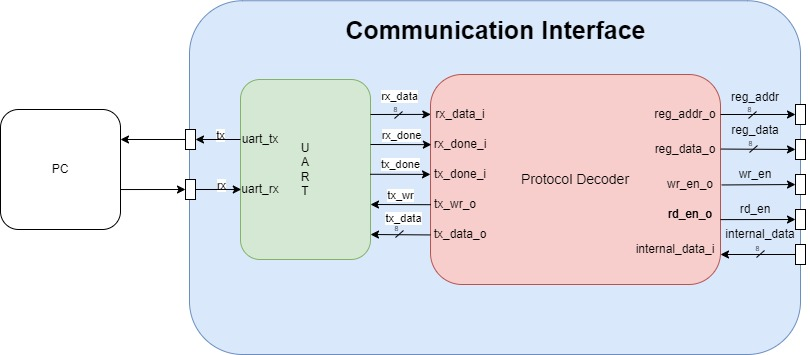
\includegraphics[width=10cm]{fig9.jpg}
			\caption{Kommunikációs interfész blokkdiagram. Az ábrát szerkesztette a szerző.  }
		\end{figure}
	
		Ez a protokoll a következőképpen működik.
		A szoftverben összeállítunk egy három, egyenként 8 bitből álló csomagot. Ennek a csomagnak az első bájtja a parancs (command) bájt, ezt követi a cím (address), végül az adat (data). Ezeket mindig egy csomagban küldjük el. 
		Az command parancsunk kétféle lehet, írás $(COM_WR)$ vagy olvasás $(COM_RD)$, ez dönti el, hogy írni vagy éppen olvasni szertnénk a regiszterfájlokat/regiszterfájlokból.
		Az cím adatunk a regiszter fájlok címét jelzi, amibe írni szeretnénk a soron következő 
		A protokoll hullámformája a következőképpen néz ki:
		\begin{figure}[h!]   %[] a kép pozíciója, h! ahova írva van a kódban ott jelenjen meg
			\centering
			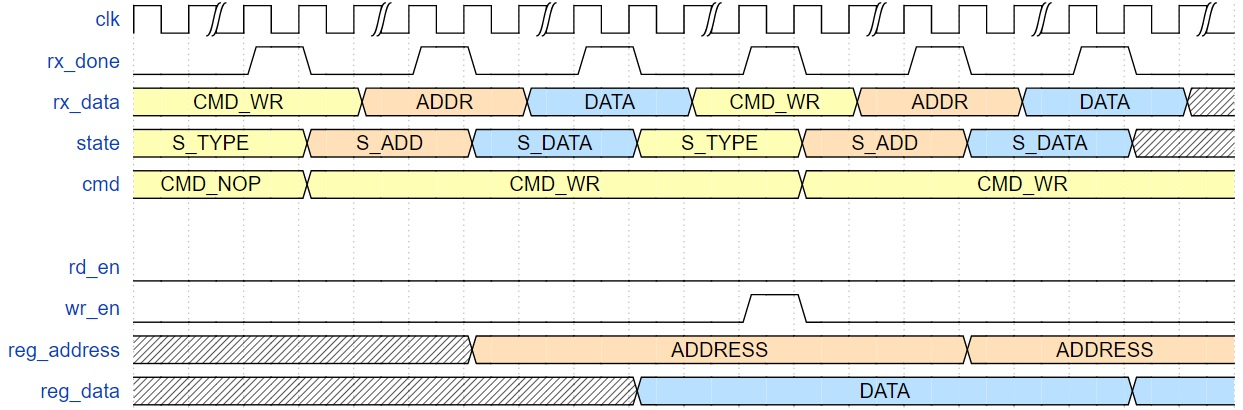
\includegraphics[width=10cm]{fig10.jpg}
			\caption{Kommunikációs protokoll hullámformája. Az ábrát szerkesztette a szerző. }
		\end{figure}
		Az modul folymatosan várja az adatokat és egy kezdő állapotból $(S_TYPE)$ indul ki, ami vizsgálja, hogy milyen parancs érkezett a bemeneten. Akkor vizsgálja meg, hogy írás vagy olvasás, mikor az $rx_done_i$ jelet megkapta, ami az UART felöl jön és akkor ad egy egy órajel szélességű impulzust mikor végzett az UART az aktuális adat olvasásával. A következő órajelre a következő állapotba lépünk, ami az $S_ADD$ állatpot, ez következő $rx_done_i$ hatására átadja az aktuális adatot az address regiszternek, melyben a megcímzendő regiszter címét tároljuk. Ezután átlépünk az $S_DATA$ állapotban. Itt megvizsgáljuk, hogy írás vagy olvasás parancsot kaptunk, ha olvasás, akkor az UART-nak átadjuk a belső regiszterből jövő adatot, ha írás akkor az UART felöli adatot adjuk át a regiszter fájlnak. Az address hatására kiválasztódik a regiszter, amibe ezt az adatot tudjuk tárolni. Majd az adat betöltése után újra a kezdő állapotba ugrunk $(S_TYPE).$
		Ennek az állapotgépnek az ún. állapotgráfját a következő ábrán láthatjuk. 
		\begin{figure}[h!]   %[] a kép pozíciója, h! ahova írva van a kódban ott jelenjen meg
			\centering
			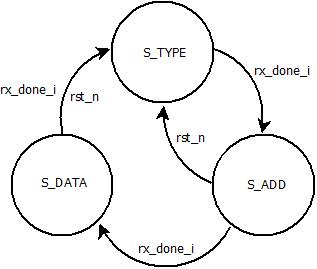
\includegraphics[width=10cm]{fig11.jpeg}
			\caption{Protokoll dekóder állapotgráf. Az ábrát készítette a szerző.}
		\end{figure}
		
		\subsection{Regiszterfájl}
		A regiszterfájl az NCO-t működtető adatok tárolására szolgál. Ennek kettős szerepe van. Az egyik ilyen, hogy eltárolja és továbbítsa a szükséges beállításokat az NCO felé, a másik pedig az, hogy leválasztja az fő funkciót, vagyis az NCO-t a kommunikációs protokolltól, tehát ha a kommunikációs protokoll megváltozik, például valami miatt egy másik fajta kommunikációval akarjuk helyettesíteni a soros kommunikációt, akkor a rendszer többi részén nem kell változtatni.  
		\begin{figure}[h!]   %[] a kép pozíciója, h! ahova írva van a kódban ott jelenjen meg
			\centering
			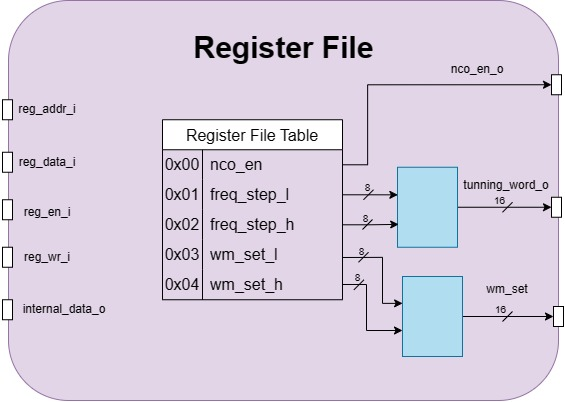
\includegraphics[width=10cm]{fig12.jpg}
			\caption{Regiszter fájl interfészei és a benne tárolt adatok. Az ábrát készítette a szerző. }
		\end{figure}
		Ebben a modulban három adatot tárolunk:
		\begin{itemize}
			\item az nco engedélyezése, ezt 1 bites regiszterben
			\item dac adatainak beállítása, ez egy 16 bites regiszterfájlban történik. Ebbe a regiszterbe a kodek beállításaihoz használt digitális szót írjuk, melyet I2C kommunikáción keresztül küldünk el az áramkörhöz
			\item tunning word, vagyis a frekvencia beállítására szolgáló adatot, ezt pedig egy 10 bites regiszterben, ami annyit jelent, hogy csak két részletben tudunk ebbe a regiszterbe írni. Ezért ítt olyan megoldáshoz kellett folyamodni, ahol szoftveresen két 8 bites adatra választjuk szét ezt a szót, majd eküldjük az UART-on, fogadjuk és két 8 bites regiszterbe írjuk őket, miután ezzel végeztünk összefűzzök egyetlen 10 bites regiszterbe ezt a két adatot. 
		\end{itemize}
	
		\subsection{Numerically Controlled Oscillator modul}
		Ez az a modul, ami a digitális hullámformát állítja elő. A bemenetére kap egy tunning word-öt, amit a számlálóhoz mindig hozzáad. Ennek elvéről az Irodalomkutatásban esett szó. Itt a megvalósításáról szeretnék pár mondatot írni. A modell blokkvázlata a következő:
		\begin{figure}[h!]   %[] a kép pozíciója, h! ahova írva van a kódban ott jelenjen meg
			\centering
			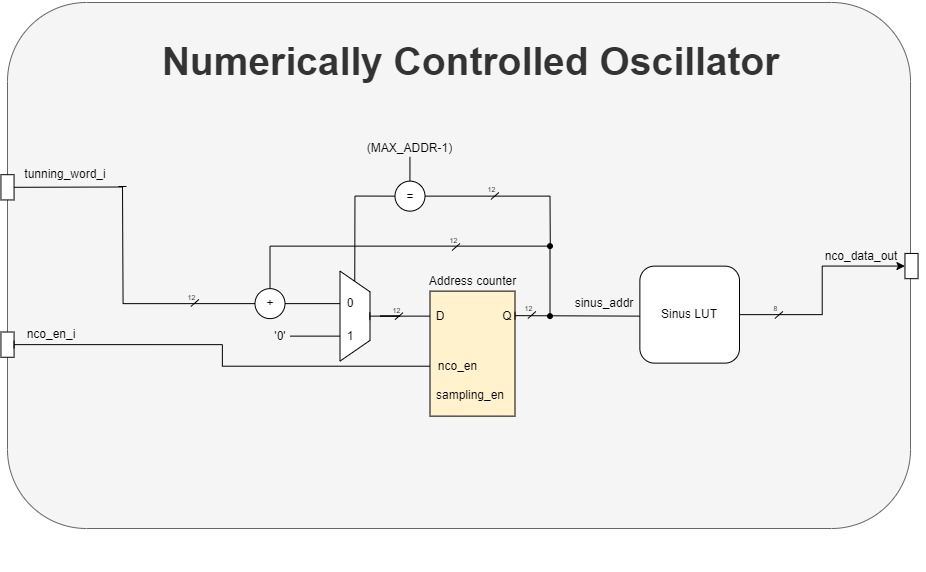
\includegraphics[width=10cm]{fig13.jpg}
			\caption{NCO blokkdiagram. Az ábrát készítette a szerző.}
		\end{figure}
		Ez egyrészt áll egy \textit{strobe} generátorból, mely egy egy órajel hosszúságú impulzust állít elő minden 520-adik órajelre, ez onnan jön, hogy 96kHz mintavételi frekvenciát szeretnénk és 50MHz-es órajel áll rendelkezésünkre, így 50MHz/520 = 96kHz.
		Ez engedélyezi mindig a számlálót, vagyis a fázis akkumulátort (phase accumulator), amihez minden egy lépésben hozzáadjuk a lépésközt. Így előáll a kimeneti cím, amit az ebben a modulban létrehozott almodulra kötünk, ez az almodul a szinusz tábla, melyet egy blockram valósít meg, aminek az eltárolt adatait megcímezve és kiolvasva rákötünk a kimenetre és előáll a szinusz jelünk.
		Az NCO bemenetén kap egy engedélyező jelet és egy frekvencialépést. Amikor az engedélyező jel ‘1’ állapotban van, akkor a rendszer kilép az alap $(S_IDLE)$ állapotba és átmegy a működési állapotába $(S\_RUN)$. Itt megvizsgálja, hogy van-e a frekvencialépés bemenetén adat, vagyis nem nulla ez a bemenet. Ha ez a bemenet nulla, akkor átlép egy $S\_WAIT$ állapotba és addig ott marad, amíg nem kapja meg a bemenetére ezt a frekvencialépést. Ezt folyamatosan, minden órajelre megvizsgálja. 
		
		\subsection{Block Ram modul}
		A ram modult szinusz táblaként használjuk, melyben eltároljuk a szoftveresen előállított hullámforma adatait. Ezek az adatok 8 bitesek. A tábla maga 12-bit mélységű, vagyis 4096 adatot tudunk benne tárolni. 
		A modul inicializálásakor a \$readmemb függvénnyel töltjük fel az adatokat, amelyeket a modul eltárol. Ez lehetővé teszi, hogy az adatok automatikusan betöltődjenek a modulba, amikor az először működik, ez csak a szimuláció során lehetséges. A szintéziskor a feltöltést máshogy kell megoldanunk, amiről a szintézis fejezetben lesz szó, lásd ~{sec: Verifikáció és szintézis}.~ fejezet.
		\begin{figure}[h!]   %[] a kép pozíciója, h! ahova írva van a kódban ott jelenjen meg
			\centering
			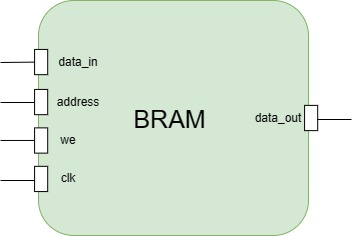
\includegraphics[width=10cm]{fig14.jpg}
			\caption{Block RAM modul interfésze. Az ábrát készítette a szerző.}
		\end{figure}
		A RAM modulja a következő módon kell kinéznie úgy, hogy azt a szintézistool felismerje és blockram-ként szintetizálja.
		\begin{lstlisting}[language=Verilog]
module sinus_lut #(
	parameter ADDR_WIDTH = 11,
	parameter DATA_WIDTH = 8,
	parameter DEPTH = 4096
)(
	input 	wire clk,
	input 	wire we,
	input 	wire  [(ADDR_WIDTH - 1) : 0] addr,
	input 	wire  [(DATA_WIDTH - 1) : 0] data_in,
	output 	logic [(DATA_WIDTH - 1) : 0] data_out
);			
logic [(DATA_WIDTH - 1) : 0] content [0 : (DEPTH-1)];
initial begin
	$readmemb("sin_lut_data.txt", content);
end
always_ff @ (posedge clk) begin
	if ( we ) content[addr] <= data_in;
end	
assign data_out = content[addr];
endmodule
		\end{lstlisting}
		Az $ADD\_WIDHT$ a címbusz bitjeinek száma, a $DATA\_WIDTH$ az adatbitek száma, a DEPTH pedig a memória mélysége. Gyakorlatilag ezzel a kódsorral hozzuk létre a memóriát, amely 8 4096 $(2^{12})$ darab 8 bites regiszterből áll. A továbbiakban pedig a memóriaregiszterek írásának és olvasásának működését adjuk meg.
		\subsection{Digitál-Analóg átalakító}
		Ahhoz hogy a digitális jelünket analóggá alakítsuk át szükségünk van egy Digitál-Analóg átalakító áramkörre, ami az Altera DE2 board-on megtalálható. Ez egy WM8731 24-bites sigma-delta audio CODEC. Ennek az áramkörnek a következő ábrán látszik a rajza, amit az altera DE2 adatlapjáról vettem át [].
		\begin{figure}[h!]   %[] a kép pozíciója, h! ahova írva van a kódban ott jelenjen meg
			\centering
			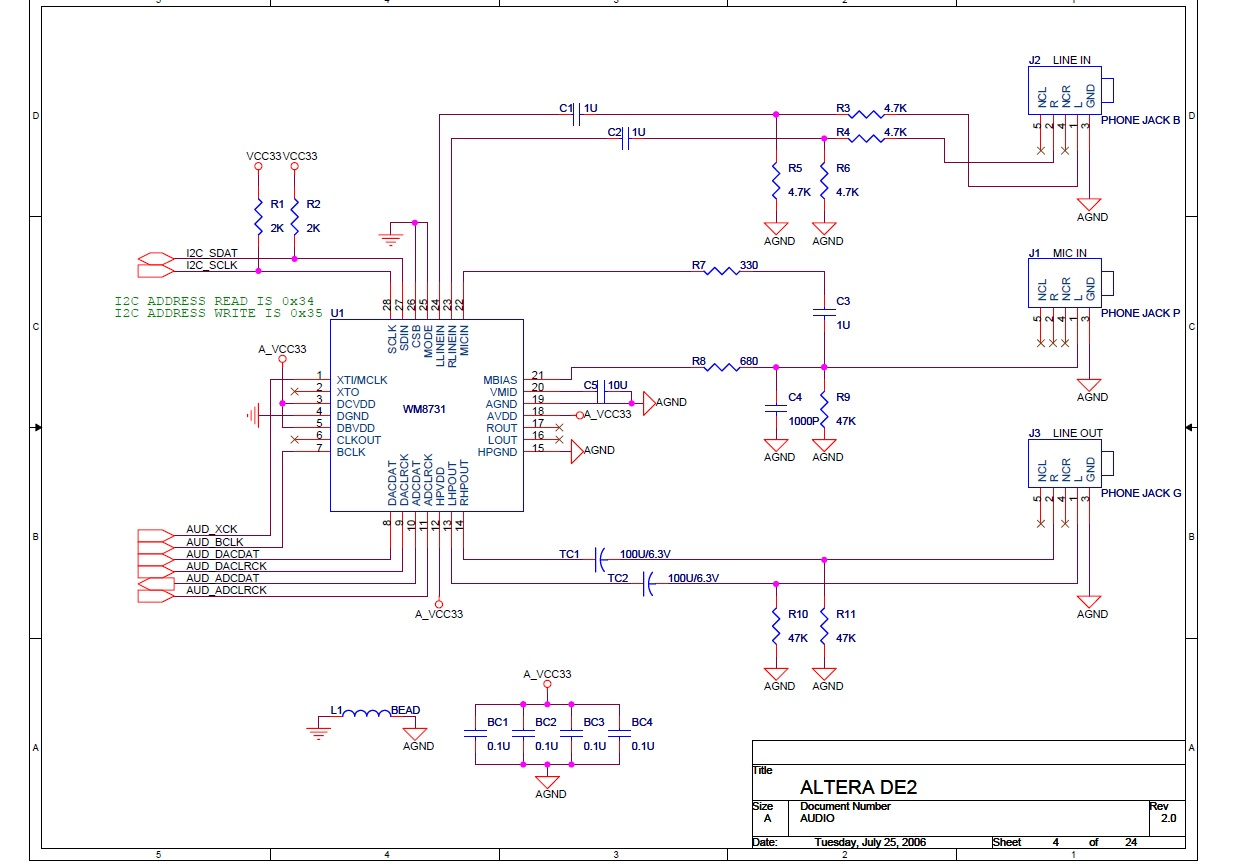
\includegraphics[width=10cm]{fig15.jpg}
			\caption{WM8731 kapcsolási rajza. A kép forrása\cite{fig15_wm8731}}
		\end{figure}
		
		A WM8731 beállításait az I2C interfészen keresztül tudja kommunikálni. Az I2C (Inter-Integrated Circuit) egy szinkron soros kommunikációs protokoll. Ez alapvetően két vezetéket használ: SDA (Serial Data) és SCL (Serial Clock). Az SDA a kétirányú adatvonal, ahol az adatok továbbítása történik. Az SCL a szinkronizációs órajelvonal, amely szabályozza az adatok átvitelének sebességét és időzítését.
		Az I2C rendszerben általában van egy központi eszköz, amelyet mesternek (master) nevezünk, és több perifériás eszköz, amelyeket szolgának (slave) hívunk. A mester irányítja az adatátvitelt a szolgákkal, és az eszközök címzése segítségével kommunikálnak egymással.
		Az I2C protokoll lehetővé teszi a soros adatok továbbítását, a multimaszter működést (több mester), az eszközök címzését, adatok olvasását és írását, valamint az eszközökkel való szinkronizációt.
		Jelen alkalmazásban a mester az FPGA és egy szolga van, ami a WM8731 kodek.
		A WM8731 adatlapjában megtalálhatók azok a regiszterek és azok a bitek, amelyeket be kell állítani a megfelelő működéshez. 
		A következő lépésekkel lehet I2C segítségével kommunikálni a WM8731 kodekkal:

		\begin{itemize}
			\item[1] Először egy Start bitet küldünk át. Az adatátviteli vonal magas állapotban van, vagyis egy lefutó él jelzi a startot.
			\item[2] Címzés: Az I2C kommunikáció során a kodeket a címével kell azonosítani. A WM8731 címe előre definiált, és a datasheet-ben megtalálható (0x35). Az FPGA elküldi a kodek címét, jelezve, hogy a további kommunikáció a WM8731 kodekkel történik.
			\item[3] Ezután beállítjuk, hogy írást vagy olvasást szeretnénk végrehajtani.
			\item[4] Majd egy ACK (acknowledgment) jelet küld a slave a master-nek
			\item[5] Regiszterek beállítása: ezután írhatunk két 8 bites adatot, melyek között szintén egy ACK jelet kapunk vissza. Ezek az adatok címzik a megfelelő regisztert, melybe beállítjuk a megfelelő biteket. Ez lehetővé teszi, hogy konfigurálhassuk a kodekünket.
			\item[6] Végül egy Stop bitet küldünk, ami jelzi az üzenet végét.
		\end{itemize}
	
		\begin{figure}[h!]   %[] a kép pozíciója, h! ahova írva van a kódban ott jelenjen meg
			\centering
			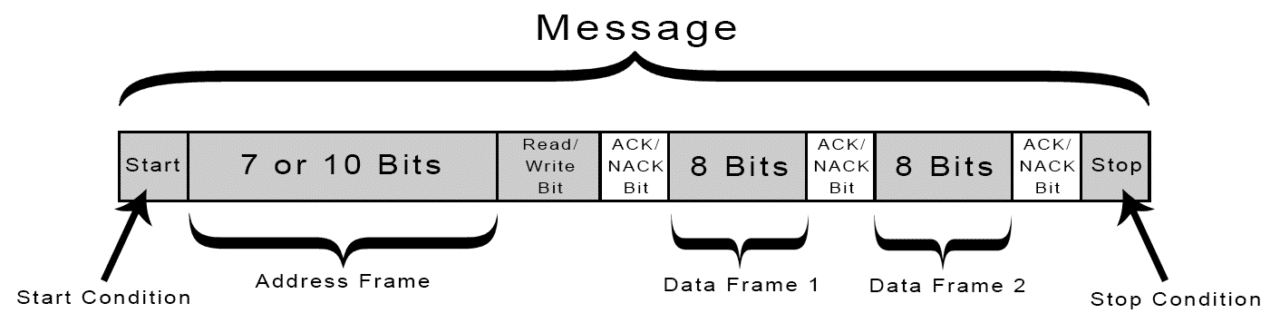
\includegraphics[width=10cm]{fig16.png}
			\caption{I2C kommunikációs protokoll. A kép forrása\cite{fig16_i2c}}
		\end{figure}
	
		Először a “0000111” című regiszter írunk, ezzel beállíthatjuk, hogy a digitális inte4rfészt DSP-vel szeretnénk vezérelni, 16 bites adatokkal és slave módban.
		Majd beállítjuk a “0000110” regiszterben, hogy a DAC-ot szeretnénk használni, az ADC-t kikaspcsoljuk. Továbbá a Linout kimenet enegedélyezését állítjuk ezzel és ráadjuk a feszültséget. Az adatokat USB módban töltjük be, ezt a “0001000” regiszterbe állítjuk. A következő lépés a “0001001” című regiszterben az aktív interfész beállítása. Utána engedélyezzük, hogy a “LINOUT” kimeneten megjelenjen a DAC kimeneti jele. Erről levesszük a némítást. Ezeket a beállításokat végrehajtva megjeleníthetjük a kimeneten a kívánt jelet.
		A beállításokat a következő táblázatban láthatjuk, ahol az első oszlop a regiszter és ennek címe, amibe szeretnénk írni. A második oszlopban a beállított adatok találhatók, a harmadikban pedig, hogy mit is állítottunk ezekkel.
		
		\begin{tabular}{|c|c|c|}
			\hline
			Regiszter címe 1 & Beírt adat  2 & Beállítások \\
			\hline
			0000111 & 000010011 & DSP mode, 16-bit data length, Right Channel DAC data when DACLRC high, Slave mode \\
			0000010 & 101111001 & Headphone volume \\
			0000110 & 000000111 & ADC off, DAC on, LINOUT on, Power on \\
			0001000 & 000000001 & USB mode(250/272fs) \\
			0001001 & 111111111 & Active interface \\
			0000100 & 000010010 & Enable DAC to LINOUT \\
			0000101 & 000000000 & Remove mute DAC \\
			\hline
		\end{tabular}
		
		Miután az átalakító beállíása megtörtént az adatok küldése egy I2S kommunikációs buszon lehetséges. Ezeket az adatokat egymás után elküldjük, amelyeket átalakít a DAC analóg jellé.  A pontos adatformátum és a küldési mód a kodek beállításától függ.
		\begin{figure}[h!]   %[] a kép pozíciója, h! ahova írva van a kódban ott jelenjen meg
			\centering
			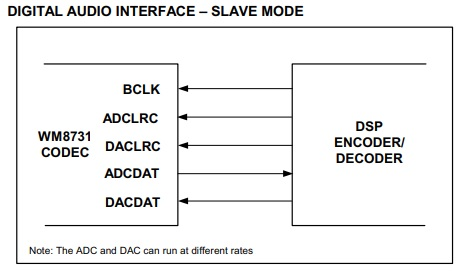
\includegraphics[width=10cm]{fig17.jpg}
			\caption{WM8731 codec I2S interfésze. A kép forrása\cite{fig17_i2s}}
		\end{figure}
		A DAC megfelelő kimeneti jelet szolgáltat egy jack csatlakozón keresztül. Ezuntán nincs más dolgunk csak mérni az adott csatlakozón a kimeneti jelet. A mérés módjáról a következő fejezetben lesz szó.
		Ezen a ponton érdemes beszélni, hogy a kimeneti digitális adatokat hogyan tudjuk illeszteni a DA konverterhez. Mivel a kimeneten egyenként 8 bites amplitúdó értékeket jelenít meg az NCO és a rendelkezésünkre álló DA átalakító 16 vagy 24 bites bitmélységgel rendelkezik (beállítástól függően), vagyis 16 bites módban 16 bites a bementi adatbusza, ezért ezeket valahogyan illesztenünk kell egymáshoz. Tehát a kérdés az, hogy mely bemenetekre kössük az egyes kimeneti vonalakat. Ezt igazából többféle módon tudjuk megtenni. Azonban a legkézenfekvőbb eset amikor a felső 8 bitre kötjük a jelet, mert ilyenkor tudjuk kihasználni a dinamikatartományt, ami nagyobb rugalmasságot és pontosságot tesz lehetővé.
		Az illesztés során az 8 bites DDS kimeneti adatokat szükséges előbb átalakítani 16 bites formátumra, hogy azokat a 16 bites DAC fogadni tudja. Ennek többféle módja van, attól függően, hogy milyen kimeneti formátumban áll rendelkezésre az DDS generátor, az egyik ilyen ismert módja az átalakításnak a nyújtás (streching). Ebben az esetben azokat az adatokat, amiket nem használunk egyszerűen kikötjük nullára. Jelen dolgozatban ezt a megoldást használtam egyszerűsége és a dinamikatartomány kihasználhatósága miatt.
		
	
		\subsection{Szoftver}
		A szoftvert Python nyleven írtam. Ez lényegében egy GUI (Graphical User Interface), ahol az adatokat tudom megadni, amivel szeretném vezérelni az FPGA-t. Ez, mint látható két részből tevődik össze, az ablak bal oldalán megadhatjuk azokat az adatokat, amiket szeretnénk beállítani. Itt megadhatjuk a DDS generátor frekvenciáját, amelyet csak 20Hz és 20kHZ között lehet megadni, ha nem ebben a tartományban adunk meg adatot, akkor a rendszer hibát dob. Továbbá a digitális-analóg átalakító beállítasait elvégző digitális szó megadása is ebben az ablakban lehetséges. Ez vár egy 16 bites bináris számot és ezt küldi el a megfelelő regiszterfájlba. 
		\begin{center}
			\textcolor{red}{
				fig18GUI kép
				Felhasználói Interfész. A képet készítette a szerző.
			}
		\end{center}
		\newpage
		Az ablak jobb oldalán a kimeneti hullámformát láthatjuk, ha a rendszerünk jól működik ez a hullámforma láthat a DDS kimmenetén, amit akár oszcilloszkóppal meg is tudunk mérni. 
		A szoftver soros porton keresztük kommunikál az FPGA-val, erre a python serial könyvtárát használtam fel. A GUI megírása a tkinter könyvtár segítségével történt.
		A hullámforma adatok generálása is ezzel a programmal történt. Először egy n elemű vektort állítottam elő mely tartalmazza az adatok sorszámát, akár a memóriacímek. Ez a vektor 14 bitméylségnek megfelelő értékű, vagyis 4096 adatot jelent. A mintavételezési frekvencia 96kHz, ebből a mintavételezési idő könnyen kiszámítható: 
		Mintavételezési idő = 1 / Mintavételi frekvencia = 1 / 96kHz = 10.42 mikroszekundum
		Ez azt jelenti, hogy a szinusz hullámforma 4096*10.42 µs = 42,680 ms időtartamú.
		Ezután eltárolom az egyes mintavételezési időpontokat, melyet úgy teszek, hogy ezt a mintavételi időtartamot megszorzom az n elemű vektor egyes vektorelemeivel. Így létrehoztuk az egyes mintavételi időpontok vektorát: xt= nt*dt
		A következő a szinusz jel létrehozása. Itt gyakorlatilag egy fázisakkumulálást hajtok végre, mivel a szinusz függvény:
		 $yt = np.cos(2*np.pi*f*xt)$, ahol
		 \begin{itemize}
		 	\item f az alap frekvenciafelbontás
		 	\item xt a mintavételezési időpontok vektora
		 	\item np olyan függvény, mely hatására egy függvény minden egyes vektorelemre külön hajtódik végre
		 \end{itemize}
	 	Ez azonban egy int típusú vektor, melyet át kell alakítani, hogy az FPGA számára is értelmezhető legyen. Az FPGA blockram-jába 8 bites kettes komplemens számokat szeretnénk tárolni. Ezért a következőképpen tudjuk a vektort átalakítani:
	 	$sin_wave = (sin_wave_int *127). astype(np.int8)$
	 	\begin{center}
	 		\textcolor{red}{
	 			fig19Python kódrészlet
	 			Hullámforma amplitúdó adatait létrehozó kódrészlet. A képet készítette a szerző.
	 		}
	 	\end{center}
	\newpage
	\section{Verifikáció és szintézis}
	Az RTL terv elkészülte után szükséges a rendszer szimulációja, hogy meggyőződjünk a megfelelő működésről mielőtt valós környzetben használnánk/ tesztelnénk az adaott áramkört.
	A rendszer tesztelésekor az volt a fő szempont, hogy megnézzük az áltanuk beírt adatok bekerültek e a regiszter fájlokba és hogy ezek alapján a kimeneti hullámformát pontosan hozzák e létre?
	A szimulációs tesztet Systemverilog nyelven terveztem és a ModelSim programmal szimuláltam. 

	Ennek eredménye a következő:

	\begin{center}
		\textcolor{red}{
			fig20Szimulációs ábra 1
			ModelSim szimuláció. Adatok írása a regiszter fájlba. A képet készítette a szerző. 
		}
	\end{center}
	Itt látható, hogy a fájlokba történő írsa sikeres volt, először az egyes állapotok váltják egymást, amint új adat érkezik be és '$rx\_done_i$' jel is kiad egy impulzust, mely azt jelzi az aktuális adat olvasása befejeződött. Továbbá látható, hogy az adott memóriacímű regiszterbe a helyes adat került. A frekvenciák összefésülése is sikeres volt.
	A következő ábrán a hullámforma szimulációja volt. Ehhez az “automatic analog” funkciót használtam, mely átalakítja a digitális adatunkat analóg hullámformává.

	\begin{center}
		\textcolor{red}{
		 fig21Szimulációs ábra 2
		 ModelSim szimuláció. A hullámforma szimulációja. A képet készítette a szerző.
		}
	\end{center}
	Először a …. Frekvencialépést adtuk meg a rendszernek, ami átszámítva a már korábban használt képlettel …frekvenciát eredményez. 
	\begin{center}
		\textcolor{red}{
			fig22Szimulációs ábra 
			ModelSim szimuláció. Periódusidő mérése. A képet készítette a szerző.
		}
	\end{center}
	Egy periódus időt megmérve és átszámítva látható, hogy a hullámforma megfelel az általunk vártnak. Később egy újabb frekvenciát írunk a regiszterbe, ezáltal megváltozik a frekvencia. Itt egy… frekvenciájú jelet látunk, ezt megmérve megfelelő működésnek a rendszerünk.  
	
	Azonban a szimuláción azt is látjuk, hogy egy frekvencia váltásnál idő kell még beáll a következő frekvenciájú állapotba a rendszer, ennek az a magyarázata, hogy 
	a két szinusz hullám összeadódásából adódik. Amikor megváltoztatjuk az NCO frekvenciáját, a kimeneti jel egy rövid időre zavaros lesz, mivel az NCO és a kimeneti jel frekvenciája közötti különbség miatt az NCO kimenete az előző és az új frekvencia közötti átmeneti időszakban átmeneti időtartam alatt változik.
	Ez az átmeneti időszak időnként a kimeneti jelben átmeneti zavarokat eredményezhet, amelyek köztes frekvenciákat jelenítenek meg a kimeneten. Ezek az átmeneti időszakok akkor is jelentkezhetnek, ha az NCO frekvenciája csak kicsit változik, vagy ha nagyobb frekvenciaugrásokat hajtunk végre.
	Ahhoz, hogy minimalizáljuk az átmeneti időszakok okozta zavarokat, az NCO frekvenciaugrásait simábbá kell tennünk. Ez általában úgy érhető el, hogy az NCO frekvenciaugrásait lineáris interpolációval simítjuk. Ebben az esetben az NCO a kimeneti frekvenciára fokozatosan áll át, és így minimalizáljuk az átmeneti időszakok okozta zavarokat.
	Másik megoldás lehet, hogy az NCO kimenetét szűrjük egy aluláteresztő szűrővel, ami elnyomja a magasabb frekvenciájú zavarokat. Az aluláteresztő szűrő általában az NCO kimeneti jelének frekvenciájától és az átmeneti időszaktól függően kerül kialakításra.
	Az átmeneti időszakok jelentősége az NCO tervezésekor és a kimeneti jel feldolgozásánál is figyelembe kell venni. A simább frekvenciaugrásokkal és az aluláteresztő szűrőkkel minimalizálhatjuk az átmeneti időszakok okozta zavarokat, így biztosítva a pontosabb és stabilabb kimeneti jel megjelenítését.
	
	A szintézis során a QUARTUS II szintézis tool-ját használtam. A szintézis során fontos megemlíteni a szinusz tábla szintetizálását. Mivel ez a tábla csak adatokat tárol, ezért az FPGA blockram memóriájaként szerettem volna szintetizálni ezt a táblát. Az adatokat a táblába a szintézis során szerettem volna betölteni. Egy .mif kiterjesztésű fájlban írattam ki az adatokat.
	DEPTH = 4096;\\
	WIDTH = 8;\\
	$ADDRESS\_RADIX$ = HEX;\\
	$DATA\_RADIX$ = HEX;\\
	CONTENT\\
	BEGIN\\
	0 : 7F;\\
	1 : 7E;\\
	.\\
	.\\
	.\\
	FFF : 7E;\\
	Mivel a memória RTL modelljét úgy írtam meg, hogy blockram-ként szintetizálja a szintézis tool, ezért ezzel már ne volt külön dolgom. A .mif fájl hozzá kellett adni a projekthez és beállítani, hogy a blockram-ba töltse be ezeket az adatokat. A szintézis sikeresen zárult.
	\begin{center}
		\textcolor{red}{
			fig23Szintézis ábra
			Hullámforma generátor szintézise. A képet készítette a szerző.
		}
	\end{center}
	\newpage
	
	\section{Áramkör mérése és mérési eredmények kiértékelése}
	Az általam használt Altera DE2 board-on megtalálható DAC megadott SFDR adata a következőképpen alakul:\\
		\textbf{\underline{A mérés célja:}}\\
		A DDS elven működő digitális hulláforma generátor tulajdonságainak meghatározása és összehasonlítás az előre meghatározott követelményekkel. Az esetleges eltérések vizsgálata, hogy mi az eltérés oka és hogy javítható-e és ha igen hogyan tudjuk ezt megtenni.\\
		\underline{A generátor előre meghatározott adatai:}
		\begin{itemize}
			\item\textbf{órajelfrekvencia:} fclk= 50MHz
			\item\textbf{mintavételi frekvencia (belső órajel):} fs = 96kHz 
			\item\textbf{DA konverter felbontása:} 16-bit 
			\item\textbf{DA konverter mintavételi sebessége:}    xxx
			\item\textbf{DA konverter SFDR értéke:}  xxx
		\end{itemize}
		Ezekből az adatokból és a mérésekből már meghatározhatóak a generátorunk paraméterei.\\
		\textbf{\underline{Frekvenciatartomány mérése:}}\\
		Az általam meghatározott frekvenciatartomány 20Hz-20kHz. Ezt mérhetjük úgy, hogy frekvenciát változtatjuk egészen 20Hz-től 20kHz-től. Ezen a tartományon belül kirajzolódik egy Bode-diagram és ha megfelelő értékű adataink vanna, vagyis nincs jelentős csillapítás az adott szakaszon (törésponti frekvencia), akkor a függvénygenerátor az adott frekvenciatartományban képes üzemelni.
		Mivel a szoftverben tetszőleges frekvenciát beállíthatunk a megadott frekvenciatartományban és a rendszer ehhez kiszámolja a szükséges frekvencialépést, amit kerekít egész számra és így a kimeneti frekvencia csak egy adott pontossággal, felbontással határozható meg. Az eltárolt adatok száma hatással lehet a fázisakkumulátor felbontására, ami pedig hatással van a maximális frekvenciatartományra. A fázisakkumulátor felbontása a mintavételi frekvencia és az eltárolt adatok száma arányának megfelelően számítható: A frekvencia felbontása tehát ismert:\\ 
		\begin{center}
			Felbontás [Hz]=fázisakkumulátor felbontása [Hz] = $\frac{96\,kHz}{2^{12}} \approx 24\,Hz$,
		\end{center}
		vagyis maximum 24Hz-es eltérés lehet a kívánt frekvencia és a tényleges frekvencia között, ez vagyis maximum 24Hz-es eltérés lehet a kívánt frekvencia és a tényleges frekvencia között, ez természetesen nagyonn mintavételi frekvenciával vagy nagyobb tárhellyel javítható.  Viszont ha pontosan 24Hz-enként nézzük végig a kimeneti jelet és mérjük a frekvenciát, akkor pontos elméletben pontos adataink lennének. Persze ez sokféle zaj és zavaró tényező befolyásolja. \\
		\textit{\underline{Mérés módja:}}\\
		Minimális frekvenciáról haladva megnézzük azt a maximális frekvenciaértéket, melynél a generátor már nem képes stabil jelet szolgáltatni. A frekvenciát 23Hz-től egészen 44kHz-ig próbáljuk változtatni mindig egy nagyságrendet haladva egészen 20Hz-ig utána pedig kisebb lépésekben.\\
		\textit{\underline{Mérési eredmények és következtetés:}}\\
		Hogy megtudjuk ezek a zajok mennyire befolyásolják a generrátorunkat meg kell határoznunk mekkora az SFDR érték. \\
		\textbf{\underline{SFDR mérése:}}\\
		\textit{\underline{Mérés módja:}}\\
		Ezt a tulajdonságot egy spektrumanalizátorral érdemes megmérni. Itt láthatóvá válik mekkora a különböző frekvenciáknál az beállított frekvenciájú komponens és a legnagyobb zaj komponens közötti különbség, vagyis a zajmentes dinamikatartomány.\\
		\textit{\underline{Mérési eredmények és következtetés:}}\\
		\begin{center}
			A mérés ábrája.
		\end{center}
		\textbf{\underline{Jitter mérése:}}\\
		\textit{\underline{Mérés módja:}}\\
		A Jitter mérésére több módszer is létezik, én az úgynevezett szemábra mérését választotta. Ennek segítségével vizuálisan megjeleníthető a jelek időzítési ingadozása. A szemábra egy időben modulált jel több ciklusát mutatja meg, ahol a jelek egymásra rakódnak. Az Eye Diagram segítségével könnyen felismerhetők a jel időzítési hibái és a jitter jellemzői.\\
		\textit{\underline{Mérési eredmények és következtetés:}}\\
		\begin{center}
			A mérés ábrája.
		\end{center}
		\textbf{\underline{Frekvencia ugrás:}}\\
		Milyen gyorsan vált át az jelünk egy másik frekvencia értékre és közte milyen zajok jelennek meg?\\
		\textit{\underline{Mérés módja:}}\\
		Első lépésben be kell állítani a DDS-t a kiindulási frekvenciára, amelyről a frekvenciaugrást szeretnénk mérni.
		Ezután beállítjuk a célfrekvenciát a célfrekvenciát, amelyre a DDS-t szeretnéd ugratni. 
		Rögzíteni szükséges a kiindulási frekvenciánál a jel spektrumát vagy frekvenciamérését a spektrumanalizátorral vagy frekvenciamérővel.
		Győződjünk meg róla, hogy a frekvenciaugrás során a DDS a lehető leggyorsabban és stabilan vált a célfrekvenciára.
		Rögzítsük és figyeljük meg a célfrekvenciánál a jel spektrumát vagy frekvenciamérését.
		Az eredményekből következtethetünk az ugrás gyorsaságára, a két beállított érték közötti megjelenő nem kívánt frekvenciákra.
		
		\textit{\underline{Mérési eredmények és következtetés:}}\\
		
		\begin{center}
			A mérés ábrája.
		\end{center}
%----------------------------------------------------------------------		
	\newpage
	%Összefoglalás
	\section{Összefoglalás}\label{sec:Összefoglaló}
	Ide jön még egy összegzés...
	\newpage
	
	%Irodalomjegyzék
	%\makeatletter
	\clearpage
	\phantomsection
	\addcontentsline{toc}{section}{Irodalomjegyzék}
	\renewcommand{\bibsection}{\section*{\bibname}}
	%\makeatother
	\bibliography{src/mybibfile.bib}

\end{document}

%Példa ábrák beillesztésére 
%\begin{figure}[h!]   	%[] a kép pozíciója, h! ahova írva van a kódban ott jelenjen meg
%\centering	   			%középre
%\includegraphics[width=10cm]{sch.png}
%\caption{Schematic}
%Forrás példa
%\cite{forrás_neve}   %bibfájlban van megadva







